\documentclass[11pt]{article}
\usepackage[left=1mm, right=1mm, top=1mm, bottom=1mm,paperwidth=140mm, paperheight=297mm]{geometry}
\usepackage[utf8]{inputenc}
\usepackage[ngerman]{babel}
\usepackage{amssymb,amsmath,amsthm,amsfonts}
\usepackage{graphicx}
\usepackage{xcolor}
\usepackage[most]{tcolorbox}
\usepackage{physics}
\usepackage{multicol}
\usepackage{tabularx}
\usepackage{relsize}
\usepackage{hyperref}
\usepackage{relsize}

\usepackage{enumitem}
\usepackage{longtable}

\title{Analysis II}
\author{}
\date{\today}

\graphicspath{ {images/} }
\setlength\parindent{0pt}
\renewcommand{\arraystretch}{1.1}
\newcommand{\sadface}{\vspace{1cm}\begin{center}\begin{Huge}:(\end{Huge}\end{center}\vspace{1cm}}
\newcommand{\sadfaces}{\vspace{1cm}\begin{center}\begin{Huge}\rotatebox{240}{:,-(}~~~~~\rotatebox{270}{:'-(}~~~~~\rotatebox{300}{:'-(}\end{Huge}\end{center}\vspace{1cm}}
\newcommand{\rom}[1]{\uppercase\expandafter{\romannumeral #1\relax}}
\newcommand\abstand{\hspace{0.5cm}}
% Bruno Eckmann (nicht weiterverwenden)
\tcbuselibrary{breakable}

\newcommand*{\Matlab}{\textsc{matlab}}
\newcommand*{\R}{\mathbb{R}}
\newcommand{\vek}[3]{\begin{pmatrix} #1 \\ #2 \\ #3 \end{pmatrix}}
\newcommand{\vekk}[2]{\begin{pmatrix} #1 \\ #2\end{pmatrix}}
\DeclareMathOperator\cis{cis}

\newcommand\Sum{\sum\limits}
\newcommand\Lim{\lim\limits_}
\newcommand\LimNI{\Lim{n \rightarrow \infty}}
\newcommand\LimNO{\Lim{n \rightarrow 0}}
\newcommand\LimXI{\Lim{x \rightarrow \infty}}
\newcommand\LimXO{\Lim{x \rightarrow 0}}
\newcommand\Int{\int\limits}

\newtcbtheorem[]{Definition}{Definition}{
	enhanced,
	breakable,
	pad at break=1mm,
	break at=-\baselineskip/0pt,
	sharp corners,
	attach boxed title to top left={
		yshifttext=-1mm
	},
	colback=white,
	colframe=blue!25!white,
	fonttitle=\bfseries,
	coltitle=black,
	before skip=10pt,
	after skip=10pt,
	boxed title style={
		sharp corners=south,
		size=small,
		colback=blue!25!white,
		colframe=blue!25!white,
	} 
}{def}

\newtcbtheorem[]{Satz}{Satz}{
	enhanced,
	breakable,
	pad at break=1mm,
	break at=-\baselineskip/0pt,
	sharp corners,
	attach boxed title to top left={
		yshifttext=-1mm
	},
	colback=white,
	colframe=magenta!25,
	fonttitle=\bfseries,
	coltitle=black,
	before skip=10pt,
	after skip=10pt,
	boxed title style={
		sharp corners=south,
		size=small,
		colback=magenta!25,
		colframe=magenta!25,
	} 
}{stz}

\newtcbtheorem[no counter]{Diverses}{Nützliches}{
	enhanced,
	breakable,
	pad at break=1mm,
	break at=-\baselineskip/0pt,
	sharp corners,
	attach boxed title to top left={
		yshifttext=-1mm
	},
	colback=white,
	colframe=magenta!25,
	fonttitle=\bfseries,
	coltitle=black,
	before skip=10pt,
	after skip=10pt,
	boxed title style={
		sharp corners=south,
		size=small,
		colback=magenta!25,
		colframe=magenta!25,
	} 
}{divs}

\newtcbtheorem[]{Rezept}{Rezept}{
	enhanced,
	breakable,
	pad at break=1mm,
	break at=-\baselineskip/0pt,
	sharp corners,
	attach boxed title to top left={
		yshifttext=-1mm
	},
	colback=white,
	colframe=yellow!55,
	fonttitle=\bfseries,
	coltitle=black,
	before skip=10pt,
	after skip=10pt,
	boxed title style={
		sharp corners=south,
		size=small,
		colback=yellow!55,
		colframe=yellow!55,
	} 
}{rzpt}

\newtcbtheorem[no counter]{Rechenregeln}{Rechenregeln}{
	enhanced,
	breakable,
	pad at break=1mm,
	break at=-\baselineskip/0pt,
	sharp corners,
	attach boxed title to top left={
		yshifttext=-1mm
	},
	colback=white,
	colframe=magenta!25,
	fonttitle=\bfseries,
	coltitle=black,
	before skip=10pt,
	after skip=10pt,
	boxed title style={
		sharp corners=south,
		size=small,
		colback=magenta!25,
		colframe=magenta!25,
	} 
}{stz}

\newtcbtheorem[]{Beispiel}{Beispiel}{
	enhanced,
	breakable,
	pad at break=1mm,
	break at=-\baselineskip/0pt,
	sharp corners,
	attach boxed title to top left={
		yshifttext=-1mm
	},
	colback=white,
	colframe=green!25,
	fonttitle=\bfseries,
	coltitle=black,
	before skip=10pt,
	after skip=10pt,
	boxed title style={
		sharp corners=south,
		size=small,
		colback=green!25,
		colframe=green!25,
	} 
}{bsp}

\newtcbtheorem[]{Quiz}{Quiz}{
	enhanced,
	breakable,
	pad at break=1mm,
	break at=-\baselineskip/0pt,
	sharp corners,
	attach boxed title to top left={
		yshifttext=-1mm
	},
	colback=white,
	colframe=red!35,
	fonttitle=\bfseries,
	coltitle=black,
	before skip=10pt,
	after skip=10pt,
	boxed title style={
		sharp corners=south,
		size=small,
		colback=red!35,
		colframe=red!35,
	} 
}{quiz}

% lean settings
% \let\olditemize=\itemize \let\endolditemize=\enditemize \renewenvironment{itemize}{\olditemize \itemsep0em}{\endolditemize}

\begin{document}

\begin{center}
\begin{Huge}Analysis II\end{Huge}\\
\end{center}

\vspace{-2em}
\section{Allgemein}

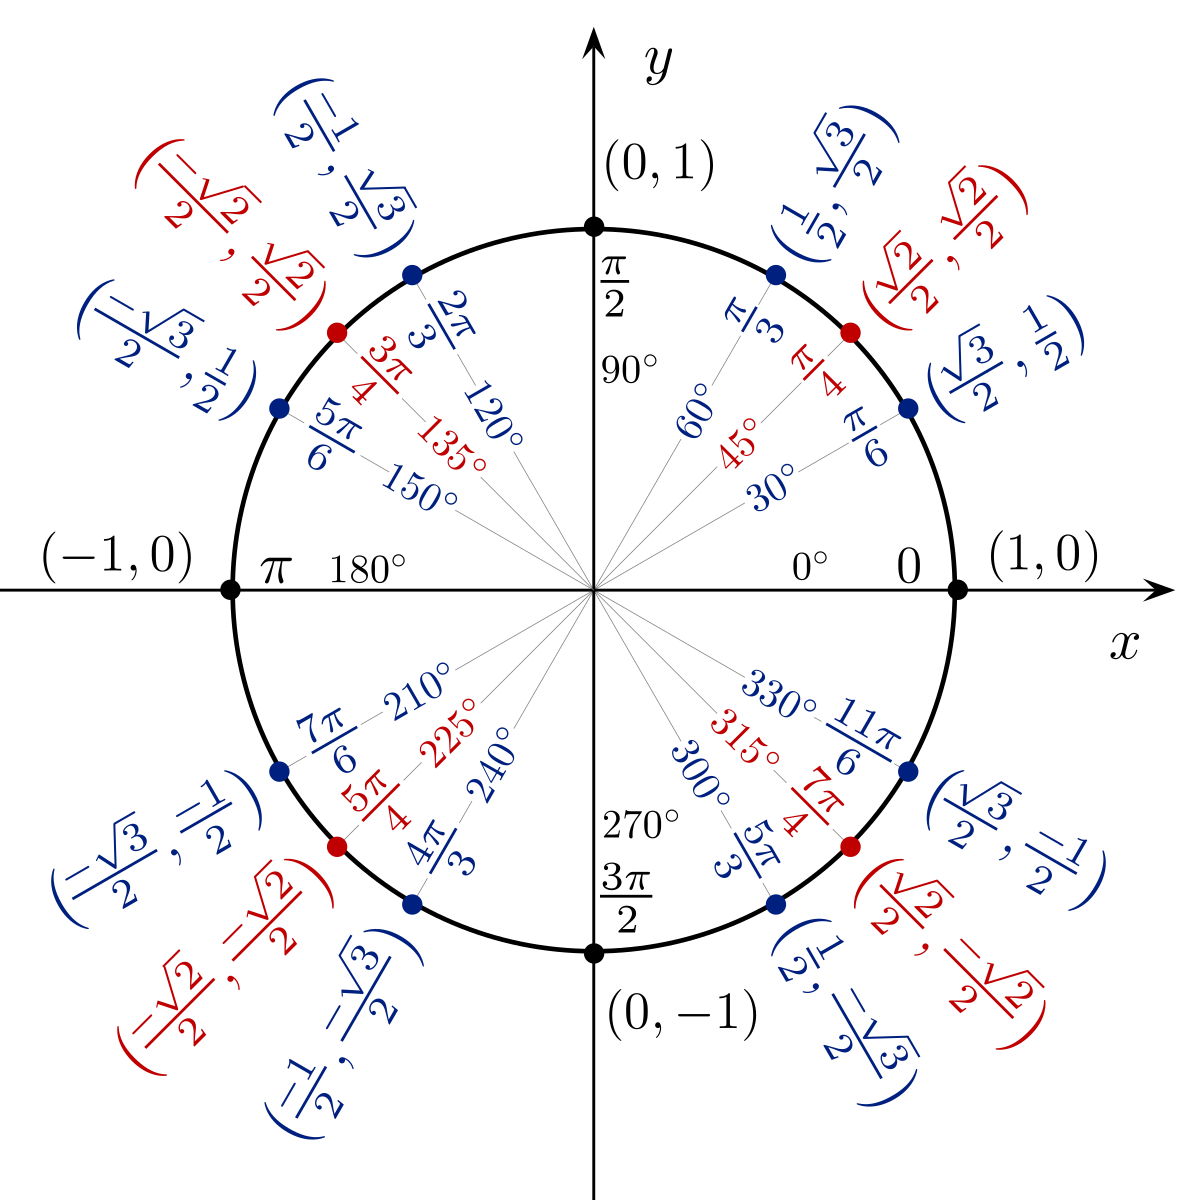
\includegraphics[width = 18em]{kreis}
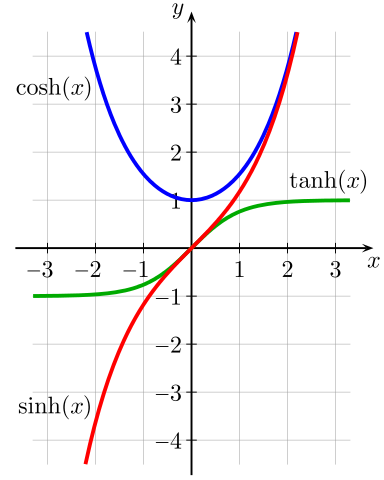
\includegraphics[width = 18em]{hyp}

\begin{Rechenregeln}{Rechenregeln Komplexe Zahlen}{}
    Imaginäre Einheit: \(i^{2} = -1\) \\
    Eulersche Formel: \( e^{i\varphi} = \cos(\varphi) + i\sin(\varphi) \), \(e^{i\varphi} = \cis(\varphi)\), \(\vert e^{i\varphi}\vert = 1\)	\\
    \begin{tabular}{|l|l|l|}
        \hline
        \(z\) & $ z = x + iy  \left\{
        \begin{array}{l}
        \text{x: Realteil}\\ \text{y: Imaginärteil}
        \end{array}
        \right. $  & \(z = r \cdot e^{i\varphi} = r \cdot \cis(\varphi)  \)\\ 
        \hline
        \(\overline{z}\) & \(\overline{z} = x - iy\) & \(z = r \cdot e^{-i\varphi}\)\\ 
        \hline
        \(\vert z \vert\) & \(\vert z \vert = \sqrt{z \cdot \overline{z}} = \sqrt{x^{2} + y^{2}}\) & \(\vert z \vert = r =\sqrt{z \cdot \overline{z}}\)\\ 
        \hline
        \(z_1 + z_2\) & \(x_1+x_2 + i(y_1+y_2)\) & \\
        \hline
        \(z_1 - z_2\) & \(x_1-x_2 + i(y_1-y_2)\) & \\
        \hline
        \(z_1 \cdot z_2\) & \((x_1x_2 - y_1y_2) + i(x_1y_2 + x_2y_1)\) & \(r_1 \cdot r_2 \cdot 
        e^{i(\varphi_1+\varphi_2)}\)\\
        \hline
        \(\frac{z_1}{z_2}, z_2 \neq 0\) & \(\frac{z_1 \cdot \overline{z_2}}{\vert z_2 \vert ^{2}} = \frac{(x_1x_2+y_1y_2)+i(x_2y_1-x_1y_2)}{x_2^{2}+y_2^{2}} \) & \(\frac{r_1}{r_2} \cdot e^{i(\varphi_1 - \varphi_2)}\)\\
        \hline
        \(\frac{1}{z}, z \neq 0\) & \(\frac{\overline{z}}{\vert z \vert ^{2}} = \frac{(x)+iy}{x^{2}+y^{2}} \) & \(\frac{1}{r} \cdot e^{-i\varphi}\)\\
        \hline
    \end{tabular}\\
    \begin{tabular}{|l|l|}
        \hline
        \(z^{n}\) & \(r^{n} \cdot (\cos(n\cdot \varphi)+ i \sin(n \cdot \varphi)) = r^{n} \cdot e^{in\varphi}\)\rule{0pt}{2.6ex}\\
        \hline
        \(\sqrt[n]{z}\) & \(\sqrt[n]{r}\cdot(\cos(\frac{\varphi + 2\pi k}{n})) + i\sin(\frac{\varphi + 2 \pi k }{n}), \ k = 0, 1, ..., n-1 \) \rule{0pt}{2.6ex}\\
        \hline
    \end{tabular}
    \begin{tabular}{|l|l|l|l|}
        \hline \(i^{0}\) & \(i^{1}\) & \(i^{2}\) & \(i^{3}\)\\
        \hline \(1\) & \(i\) & \(-1\) & \(-i\)\\
        \hline
    \end{tabular}
\end{Rechenregeln}

\begin{Rechenregeln}{Allgemeine Rechenregeln}{}
    \textbf{Betrag:} \\
    \(\vert ab \vert = \vert a \vert \vert b\vert \) \abstand 
    \(\vert \frac{a}{b} \vert = \frac{\vert a \vert}{ \vert b\vert} \) \abstand
    \(\vert a + b \vert \le \vert a \vert + \vert b \vert\) \\
    \\
    \textbf{Potenzen:} \\
    \(x = \sqrt[n]{a} 	\Leftrightarrow\ (x^{n}  = a \ \text{und } x \ \ge 0)\) \abstand
    \(\sqrt[n]{-a} = - \sqrt[n]{a}, \ a \ge 0\) \abstand
    \(a^{-n} = \frac{1}{a^{n}} = (\frac{1}{a})^{n}\) \abstand \(a^{\frac{1}{n}} = \sqrt[n]{a}\) \abstand \(\sqrt{ab} = \sqrt{a}\sqrt{b}\)\abstand \(a^{\frac{m}{n}} = \sqrt[n]{a^{m}}\) \abstand
    \( \sqrt{\frac{a}{b}} = \frac{\sqrt{a}}{\sqrt{b}} \) \abstand \( a^{x} = e^{x \cdot \ln a}\) \abstand 
    \(\sqrt[n]{a^{-m}} = \frac{1}{\sqrt[n]{a^{m}}}\)
    \(a^{m}a^{n} = a^{m+n} \) \abstand \(\sqrt[n]{a^{m}} = \sqrt[kn]{a^{km}}\) \abstand \(\frac{a^{m}}{a^{n}} = a^{m-n}\)
    \\ \( \sqrt[n]{\sqrt[k]{a}} = \sqrt[nk]{a}\) \abstand  \((a^{m})^{n} = a^{mn}\) \abstand \(\sqrt[n]{a}\sqrt[n]{b} = \sqrt[n]{ab}\) 
    \abstand \(a^{n}b^{n} = (ab)^{n}\) \abstand \(\frac{\sqrt[n]{a}}{\sqrt[n]{b}} = \sqrt[n]{\frac{a}{b}}\) 
    \abstand \(\frac{a^{n}}{b^{n}} = (\frac{a}{b})^{n}\) 
\end{Rechenregeln}

\begin{Rechenregeln}{Sinus und Cosinus}{}
    \begin{tabular}{|c@{\hspace{3pt}}|c@{\hspace{3pt}}|c|c|c|c|c|c|c|c|}
        \hline
        Grad &$0^\circ$ &$30^\circ$ &$45^\circ$ &$60^\circ$ &$90^\circ$ &$120^\circ$ &$135^\circ$ &$150^\circ$ &$180^\circ$\\
        \hline
        $\varphi$ &$0$ &$\frac{\pi}{6}$ &$\frac{\pi}{4}$ &$\frac{\pi}{3}$ &$\frac{\pi}{2}$ &$\frac{2\pi}{3}$ &$\frac{3\pi}{4}$ &$\frac{5\pi}{6}$ &$\pi$\\
        \hline
        $\sin(\varphi)$ &$0$ &$\frac{1}{2}$ &$\frac{\sqrt{2}}{2}$ &$\frac{\sqrt{3}}{2}$ &$1$ &$\frac{\sqrt{3}}{2}$ &$\frac{\sqrt{2}}{2}$ &$\frac{1}{2}$ &$0$\\
        \hline
        $\cos(\varphi)$ &$1$ &$\frac{\sqrt{3}}{2}$ &$\frac{\sqrt{2}}{2}$ &$\frac{1}{2}$ &$0$ &$-\frac{1}{2}$ &$-\frac{\sqrt{2}}{2}$ &$-\frac{\sqrt{3}}{2}$ &$-1$\\
        \hline
        $\tan(\varphi)$ &$0$ &$\frac{\sqrt{3}}{3}$ &$1$ &$\sqrt{3}$ &$\pm \infty$ &-$\sqrt{3}$ &$-1$ &$-\frac{\sqrt{3}}{3}$ &$0$\\
        \hline 
    \end{tabular}
    \begin{itemize}
    \item $\sin(x \pm y) = \sin(x)\cos(y) \pm \cos(x)\sin(y)$
    \item $\cos(x \pm y) = \cos(x)\cos(y) \mp \sin(x)\sin(y)$
    \item $\sin(x+y)\sin(x-y) = \cos^2(y) - \cos^2(x) = \sin^2(x) - \sin^2(y)$
    \item $\cos(x+y)\cos(x-y) = \cos^2(y) - \sin^2(x) = \cos^2(x) - \sin^2(y)$
    \item $\sin{x}\cos{y} = \frac{1}{2}(\sin(x+y) + \sin(x-y))$ 
    \item $\cos{x}\cos{y} = \frac{1}{2}(\cos(x+y) + \cos(x-y))$
    \item  $\sin{x}\sin{y} = \frac{1}{2}(\cos(x-y)-\cos(x+y))$
    \item $\cos(x)^2 + \sin(x)^2 = 1$
    \item $\cos(\pi-x) = -\cos(x)$, $\sin(\pi-x) = \sin(x)$
    \item $\cos(x+\pi) = -\cos(x)$, $\sin(x+\pi) = -\sin(x)$
    \item $\cos(2x) = \cos^2(x) - \sin^2(x) = 1-2\sin^2(x) = 2\cos^2(x) - 1$
    \item $\sin(2x) = 2\sin(x)\cos(x)$ \abstand $\tan(2x) = \frac{2\tan(x)}{1-\tan^2(x)}$
    \item $\sin(\frac{x}{2}) = \sqrt{\frac{1-\cos(x)}{2}}$ \abstand $\cos(\frac{x}{2}) = \sqrt{\frac{1+\cos(x)}{2}}$
    \item $\tan(\frac{x}{2}) = \frac{1-\cos(x)}{\sin(x)} = \frac{\sin(x)}{1+\cos(x)}$ \abstand $\cot(\frac{x}{2}) = \frac{1+\cos(x)}{\sin(x)} = \frac{\sin(x)}{1-\cos(x)}$
    \item $\sin^2(x) = \frac{1-\cos(2x)}{2}$
    \abstand $\cos^2(x) = \frac{1+\cos(2x)}{2}$
    \item $\sin^3(x) = \frac{3\sin(x) - \sin(3x)}{4}$ 
    \abstand $\cos^3(x) = \frac{3\cos(x) + \cos(3x)}{4}$
    \item $\tan(\pi + x) = \tan(x)$
    \item $-\sin(-x) = \sin(x), \cos(-x) = \cos(x), \tan(-x) = -\tan(x)$
    \item Für alle $(a,b)\in \R^2$, sodass $a^2+b^2 = 1$, gibt es $x\in\R$, sodass $a = \cos(x)$, $b = \sin(x)$.
    \item $\sin(x) = \frac{2\tan(x/2)}{1+\tan^2(x/2)}$
    \abstand $\cos(x) = \frac{1-\tan^2(x/2)}{1+\tan^2(x/2)}$
    \item $\sin(x) = \frac{e^{ix} - e^{-ix}}{2i}$
    \abstand $\cos(x) = \frac{e^{ix} + e^{-ix}}{2}$
    \item $\int_0^{2\pi} \sin(t)\cdot \cos(t) dt = \int_0^{2\pi} \sin(t) dt = \int_0^{2\pi} \cos(t) dt = 0$
    \item $\int \sin^2(x) dx = \frac{1}{2} (x-\sin(x) \, \cos(x))$
    \item $\int \cos^2(x) dx = \frac{1}{2} (x+\sin(x) \, \cos(x))$
    \item $\int x \sin(x) dx = \sin (x)-x \cos (x)$
    \item $\int x \cos(x) dx = x \sin (x)+\cos (x)$
    \item \(\sin(\arccos(x)) = \sqrt{1-x^{2}}\) \abstand \(\sin(\arctan(x)) = \frac{x}{\sqrt{1+x^{2}}}\) 
    \item \(\cos(\arctan(x)) = \frac{1}{\sqrt{1+x^{2}}}\) \abstand \(\cos(\arcsin(x)) = \sqrt{1-x^{2}}\) 
    \item \(\tan(\arcsin(x)) = \frac{x}{\sqrt{1-x^{2}}}\) \abstand \(\tan(\arccos(x)) = \frac{\sqrt{1-x^{2}}}{x}\)
    \item $\cosh(x) := \frac{e^x + e^{-x}}{2}$ \abstand $\sinh x := \frac{e^x - e^{-x}}{2}$ \abstand $\tanh x := \frac{e^x - e^{-x}}{e^x + e^{-x}}$
    \item $\sinh(z) = -\sinh(-z)$ \abstand $\cosh(z) = \cosh(-z)$ 
    \item $\sinh(z) = \sinh(z + 2\pi i)$ \abstand $\cosh(z) = \cosh(z+ 2\pi i)$
    \item $\sinh(z_1 \pm z_2) = \sinh(z_1) \cdot \cosh(z_2) \pm \sinh(z_2) \cdot \cosh(z_1)$
    \item $\sinh(z_1 \pm z_2) = \cosh(z_1) \cdot \cosh(z_2) \pm \sinh(z_2) \cdot \sinh(z_1)$
    \item $\tanh(z_1 \pm z_2) = \frac{\tanh(z_1) \pm \tanh(z_2)}{1 \pm \tanh(z_1)\cdot \tanh(z_2)}$
    \end{itemize}
\end{Rechenregeln}

\begin{Rechenregeln}{Ableitung}{}
    \begin{itemize}
        \item \textbf{Summenregel} $(f(x)+g(x))' = f'(x) + g'(x)$
        \item \textbf{Faktorregel} $(c\cdot f(x))' = c\cdot f'(x)$
        \item \textbf{Produktregel} $(f(x)\cdot g(x))' = f'(x)g(x) + f(x)g'(x)$
        \item \textbf{Quotientenregel} $\left(\frac{f(x)}{g(x)}\right)' = \frac{f'(x)g(x) - f(x)g'(x)}{g^2(x)}(g\neq 0)$
        \item \textbf{Kettenregel} $(f(g(x)))' = (f\circ g)' = f'(g(x))g'(x)$
    \end{itemize}
\end{Rechenregeln}

\begin{Rechenregeln}{Integration}{}
    \begin{itemize}
    \item \textbf{Summe/Differenz:} $\int_a^b (f(x) +/- g(x)) xd = \int_a^b f(x) +/- \int_a^b g(x)$
    \item \textbf{Konstanter Faktor:} $\int_a^b c\cdot f(x)dx = c\cdot \int_a^b f(x)dx$
    \item \textbf{Partielle Integration:} $\int_a^b f'(x)\cdot g(x)dx = \left[f(x)g(x)\right]_a^b - \int_a^b f(x)g'(x)$
    \item \textbf{Substitution:} $\int_{\phi(a)}^{\phi(b)} f(x)dx = \int_a^b f(\phi(t))\phi '(t) dt$
    \item \textbf{$a+c, b+c \in I$} $\int_a^b f(t+c)dt = \int_{a+c}^{b+c} f(x)dx$
    \item \textbf{$ca,cb\in I$: } $\int_a^b f(ct)dt = \frac{1}{c}\int_{ca}^{cb} f(x)dx$
    \item \textbf{Logarithmus: }\;(f stetig diffbar) $\int\frac{f'(t)}{f(t)}dt = \log(|f(x)|)$, bzw. $\int_a^b\frac{f'(t)}{f(t)}dt = \log(f(|b|)) - \log(f(|a|))$
    \item \textbf{Partialbruch: }\\
     $\frac{2x^6-4x^5+5x^4-3x^3+x^2+3x}{(x-1)^3(x^2+1)^2} = \frac{A}{x-1}+\frac{B}{(x-1)^2}+\frac{C}{(x-1)^3}+\frac{Dx+E}{x^2+1}+\frac{Fx+G}{(x^2+1)^2}$
    \end{itemize}
\end{Rechenregeln}

\begin{Rechenregeln}{Limes}{}
    \begin{itemize}
    \item $\lim_{x\to 0} \arctan(x) = 0$, $\lim_{x\to\infty} \arctan(x) = \frac{\pi}{2}$
    \item $\lim_{x\to 0} \tan(x) = 0$, $\lim_{x\to\infty} \tan(x) = \infty$, $\lim_{x\to\frac{\pi}{2}} \tan(x) = \infty$
    \item $\Lim{n \rightarrow \infty}{(1+\frac{x}{n})^{n}} = e^{x}$ \abstand $\Lim{n \rightarrow \infty}{(1+\frac{1}{n})^{n}} = \LimNI{(1+n)^{\frac{1}{n}}} = e$ 
    \item $\LimXO{\frac{a^{x}-1}{x}} = \ln(a)$ \abstand \(\LimXO\frac{\log_a(1+x)}{x} = \frac{1}{\ln(a)}\) \abstand \(\LimXO{\frac{1-\cos(x)}{x}} = 0\) 
    \item \( \LimXO{\frac{1-\cos(x)}{x^{2}}} = \frac{1}{2} \) \abstand \( \LimXO{\frac{\tan(x)}{x}} = 1\) \abstand \( \LimXO{\frac{\sin(x)}{x}} = 1 = \frac{x}{\sin(x)}\) 
    \item \(\LimNI{\frac{n!}{n^{n}}} = 0\) \abstand \(\LimNO{\frac{e^{n} -1}{n}} = 1\) \abstand \(\LimNI{\sqrt[n]{n!}} = \infty\) \abstand \(\LimNI {\sqrt[n]{n}} = 1\)
    \end{itemize}
    \textbf{Entscheidbare Situationen}
    $\frac{1}{0} = \infty$ \abstand $\frac{1}{\infty} = 0$ \abstand $\infty + \infty = \infty$ 
    \abstand $0 + \infty = \infty$ \abstand $0^{\infty} = 0$ \abstand $\infty^{\infty} = \infty$
\end{Rechenregeln}

\begin{Rechenregeln}{Reihen}{}
    \begin{itemize}
        \item $\sum_{k=0}^{\infty} aq^{k} = a + aq + aq^{2} +... = \frac{a}{1-q}$ (geometrische Reihe)
        \item $\sum_{k=0}^{\infty} (k+1)q^{k} = 1 + 2q + 3q^{2} +... = \frac{1}{(1-q)^{2}}, \ \vert q \vert < 1$ 
        \item $\sum_{k=0}^{\infty} \frac{(-1)^{k}}{2k+1} = 1 - \frac{1}{3} + \frac{1}{5} - \frac{1}{7} + ... = \frac{\pi}{4}$
        \item $\sum_{k=1}^{\infty} \frac{1}{k^{2}} = 1 + \frac{1}{2^{2}} + \frac{1}{3^{2}} + \frac{1}{4^{2}} + ... = \frac{\pi^{2}}{6}$
        \item $\zeta(a) = \sum_{k=0}^{\infty} \frac{1}{k^{a}} \text{ist konvergent} \iff a>1$
        \item $\sum_{k=0}^{\infty} \frac{1}{k!} = 1+\frac{1}{1!} + \frac{1}{2!} + \frac{1}{3!} + ... = e$
        \item $\sum_{k=0}^{\infty} \frac{(-1)^{k}}{k!} = 1 - \frac{1}{1!} + \frac{1}{2!} - \frac{1}{3!} + ... = \frac{1}{e}$
        \item $\frac{1}{1 \pm x} = 1 \mp x + x^2 \mp x^3 + x^4 \mp ...$
        \item $\frac{1}{(1 \pm x)^2} = 1 \mp 2x + 3x^2 \mp 4x^3 + 5x^4 \mp ...$
        \item $\sqrt{1 \pm x} = 1 \pm \frac{x}{2} - \frac{\scriptstyle{1\cdot 1}}{\scriptstyle{2 \cdot 4}}x^2 \pm \frac{\scriptstyle{1\cdot 1 \cdot 3}}{\scriptstyle{2 \cdot 4 \cdot 6}}x^3 - \frac{\scriptstyle{1 \cdot 1 \cdot 3 \cdot 5}}{\scriptstyle{2 \cdot 4 \cdot 6 \cdot 8}}x^4 \pm \scriptstyle\cdots$
        \item $\exp(x) = \sum_{n=0}^{\infty} \frac{x^{n}}{n!} = 1 + x + \frac{x^{2}}{2!} + \frac{x^{3}}{3!} + ....$
        \item $\sin(x) =  \sum_{n=0}^{\infty} (-1)^{n}\frac{x^{2n+1}}{(2n +1)!} = x - \frac{x^{3}}{3!} + \frac{x^{5}}{5!} - \frac{x^{7}}{7!} + ...$ 
        \item $\cos(x) =  \sum_{n=0}^{\infty} (-1)^{n}\frac{x^{2n}}{(2n)!} = 1 - \frac{x^{2}}{2!} + \frac{x^{4}}{4!} - \frac{x^{6}}{6!} + ...$ 
        \item $\sinh(x) = \sum_{n=0}^{\infty} \frac{x^{2n+1}}{(2n+1)!} = x + \frac{x^3}{3!} + \frac{x^5}{5!} + ...$
        \item $\cosh(x) = \sum_{n=0}^{\infty} \frac{x^{2n}}{(2n)!} = 1 + \frac{x^2}{2!} + \frac{x^4}{4!} + ...$
        \item $\tan(x) = 1 + \frac{x^3}{3} + \frac{2x^5}{15} + ...$
        \item $\tanh(z) = 1 \pmb{-} \frac{z^3}{3} \pmb{+} \frac{2z^5}{15} \pmb{-} ...$
        \item $\ln(1+z) = \sum_{k=1}^{\infty} \frac{(-1)^{k+1}}{k}z^k = z - \frac{z^2}{2} + \frac{z^3}{3} + ...$
        \item $(1+z)^\alpha = \sum_{k=0}^{\infty}  \binom{\alpha}{k} z^k = 1 + \alpha z + \frac{\alpha(\alpha - 1)}{2!} z ^ 2 + ...$
    \end{itemize}
\end{Rechenregeln}

\begin{Diverses}{}{}
    \begin{itemize}
    \item Kreisgleichung $(x - x_0)^2 + (y - y_0)^2 = r^2$
    \item Ellipsengleichung $\frac{(x-x_0)^2}{a^2} + \frac{(y-y_0)^2}{b^2} = 1$
    \item Mitternachtsformel $x_{1, 2} = \frac{-b \pm \sqrt{b^2 - 4ac}}{2a}$
    \item Matrix Determinante $\begin{vmatrix}
        a & b\\
        c & d
    \end{vmatrix} = ad-bc$
    \item Matrix Invertierbarkeit: Eine quadratische Matrix ist genau dann invertierbar, falls die Determinante $\neq 0$.
    \item Skalarprodukt $x \cdot y = \sum_{i=1}^n x_i y_i$
    \item Kreuzprodukt $a \times b = (a_2b_3-a_3b_2, ~~~ a_3b_1-a_1b_3, ~~~ a_1b_2-a_2b_1)^\top$
    \end{itemize}
\end{Diverses}

\begin{Rechenregeln}{Stammfunktionen, Ableitungen}{}
    \begin{center}
        $\textbf{differenzierbar }\implies\textbf{ stetig }\implies \textbf{ integrierbar}$\\
    \end{center}
    \begin{longtable}{l|l|l}
        $\mathbf{f'(x)}$ & $\mathbf{f(x)}$ & $\mathbf{F(x)}$ \\[0.5em] \hline
        0 & c ($c\in\R)$ & $cx$ \\[0.5em]
        $c$ & $cx$ &$\frac{c}{2}x^2$ \\[0.5em]
        $r\cdot x^{r-1}$ & $x^r (r\in \R \backslash \{-1\}$ & $\frac{x^{r+1}}{r+1}$ \\[0.5em]
        $\frac{-1}{x^2} = -x^{-2}$ & $\frac{1}{x}=x^{-1}$ & $\log |x| $ \\[0.5em]
        $\frac{1}{2 \sqrt{x}} = -x^{-2}$ & $\sqrt{x} = x^{\frac{1}{2}}$ & $\frac{2}{3}x^{\frac{3}{2}}$ \\[0.5em]
        $\cos x$ & $\sin x$  & $-\cos x$ \\[0.5em]
        $-\sin x$ & $\cos x$ & $\sin x$\\[0.5em]
        $1+\tan^2x = \frac{1}{\cos^2x}$ & $\tan x$ & $-\log|\cos x|$\\[0.5em]
        $-\frac{1}{\sin^2(x)}$ & $\cot x$ & $\log|\sin x|$\\[0.5em]
        $e^x$ & $e^x$ & $e^x$\\[0.5em]
        $c\cdot e^{cx}$ & $e^{cx}$ & $\frac{1}{c}e^{cx}$\\[0.5em]
        $\log a \cdot a^x$ & $a^x$ & $\frac{a^x}{\log a}$\\[0.5em]
        $\frac{1}{x}$ & $\log|x|$ & $x(\log|x|-1)$ \\[0.5em]
        $\frac{1}{\log a\cdot x}$ & $\log_a |x|$ & $\frac{x}{\log a}(\log|x|-1)$\\[0.5em]
         & & = $x(\log_a|x|-\log_ae)$\\[0.5em]
        $\frac{1}{\sqrt{1-x^2}}$ & $\arcsin x$ & $x\arcsin x + \sqrt{1-x^2}$\\[0.5em]
        $-\frac{1}{\sqrt{1-x^2}}$ & $\arccos x$ &  $x\arccos x - \sqrt{1-x^2}$\\[0.5em]
        $\frac{1}{1+x^2}$ & $\arctan x$ & $x\arctan x - \frac{1}{2}\log(1+x^2)$\\[0.5em]
        $\sinh(x)$ & $\cosh(x)$ & - \\[0.5em]
        $\cosh(x)$ & $\sinh(x)$ & -\\[0.5em]
        $\frac{1}{\cosh^2(x)}$ & $\tanh(x)$ & $\log(\cosh(x))$\\[1em]
        $2 \sin(x)\cos(x)$ & $\sin^2(x)$ & $\frac{1}{2}(x-\sin(x)\cos(x))$ \\[.5em]
        $-2\sin(x)\cos(x)$ & $\cos^2(x)$ & $\frac{1}{2}(x+\sin(x)\cos(x))$ \\[.5em]
        $\frac{2 \sin(x)}{\cos^3(x)}$ & $\tan^2(x)$ & $\tan(x) - x$\\[.5em]
        \(\frac{1}{\sqrt {x^2+1}}\)& \(\operatorname{arsinh} x\) & \(x \operatorname{arsinh} x -\sqrt{x^2+1}\)\\
        \(\frac{1}{\sqrt {x^2-1}} \quad (x>1)\)&\(\operatorname{arcosh} x\) & \(x \operatorname{arcosh} x -\sqrt{x^2-1}\)\\
        \(\frac{1}{1-x^2} \quad (\left| x \right|<1)\)&\(\operatorname{artanh} x\) & \(x \operatorname{artanh} x +\frac{1}{2}\ln{\left(1-x^2\right)}\)\\
        \(\frac{1}{1-x^2} \quad (\left| x \right|>1)\)&\(\operatorname{arcoth} x\) & \(x \operatorname{arcoth} x +\frac{1}{2}\ln{\left(x^2-1\right)}\)\\ 
    \end{longtable}
\end{Rechenregeln}


\section{Differentialgleichungen}

\begin{Definition}{Ordnung, linear, homogen}{}
    Die \textbf{Ordnung} einer Gleichung ist die höchste vorkommende Ableitung. Bsp: $y''$ $\implies$ 2.\\
    
    Eine Differentialgleichung heisst \textbf{linear}, falls jeder Term $y$, $y'$, $y''$ usw. nur linear vorkommt. Wichtig: Falls $y_1(x)$ und $y_2(x)$ Lösungen der selben Differentialgleichung sind, dass ist auch die Linearkombination $ay_1(x) + by_2(x)$.\\
    
    Eine Differentialgleichung heisst \textbf{homogen}, falls keine Terme vorkommen, die rein von den Funktionsvariablen x abhängen (also kein $x$, $\sin(x)$, ... enthalten). Sonst heisst die Gleichung \textbf{inhomogen}.
\end{Definition}

\begin{Definition}{Anfangswertproblem}{}
    Ein \textbf{Anfangswertproblem} $n$-ter Ordnung ist eine gewöhnliche Differentialgleichung $n$-ter Ordnung zusammen mit $n$ Anfangsbedingungen.
\end{Definition}


\begin{Satz}{Hauptsatz lineare Differentialgleichung}{}
	Sei $I \subset \mathbb{R}$ an offenes Interval and $k \geq 1$ eine ganze Zahl,\\
	$y^{(k)} + a_{k-1}y^{(k-1)} +... \ + a_1y' + a_0 y = 0$ eine homogene lineare ODE über $I$ mit stetigen Koeffizienten.
	Dann sind: 
	\begin{enumerate}
		\item Dann ist die Menge $S$ bestehend aus k-fach differenzierbaren Lösungen $f: I \rightarrow \mathbb{C}$ ein komplexer Vektorraum der Grösse k.
		\item Für alle Anfangswerte $(y_0, ... \ , y_{k-1}) \in \mathbb{C}^k$ gibt es eine eindeutige Lösung $f \in \mathbb{C}$ so dass $f(x_0) = y_0, f'(x_0) = y_1, ... \ , f^{(k-1)} = y_{k-1}$
		\item Sei $b$ stetig über I. Dann existiert eine Lösung $f_p$ für das inhomogene ODE und $S_b = f + f_p$
		\item Für alle Anfangswerte ist die Lösungen eindeutig.
		\item \textcolor{red}{Wenn $b \neq 0, S_b$ ist kein Vektorraum} 
	\end{enumerate}
\end{Satz}
\begin{Satz}{Grundprinzip für lineare, inhomogene Differentialgleichungen}{}
    Die allgemeine Lösung einer linearen, inhomogenen Differentialgleichung hat die Form
    \[
        \underbrace{y(x)}_{\text{Gesamtlösung}}
        = \underbrace{y_{hom}(x)}_{\text{allg. homogene Lösung}}
        + \underbrace{y_p(x)}_{\text{partikuläre Lösung}}
    \]
\end{Satz}

\begin{Rezept}{Reduktion der Ordnung}{}
	Reduktion einer ODE mit Ordnung $k$ auf Ordnung 1:
	Man definiere 
	\begin{equation*}
		f: \mathbb{R} \rightarrow \mathbb{R}^k \qquad x \longmapsto \begin{pmatrix} y(x) \\ y'(x)\\ \cdots \\ y^{(k)}(x)\end{pmatrix} \qquad
		f'(x)= \begin{pmatrix} y'(x) \\ y''(x) \\ \cdots \\ \small{\text{original equation}} \\ \small{\text{solved for $y^{(k)}(m)$}}
		\end{pmatrix}
	\end{equation*}
	
	Für $k=3$ und $ \rom{1}: y''' = cy'' + by' + ay$:
		\begin{equation*}
		f'(x)= \underbrace{\begin{pmatrix}
		0 & 1 & 0 \\ 0 & 0 & 1 \\ a & b & c
		\end{pmatrix}}_{A(x)} \cdot \begin{pmatrix} y(x) \\ y'(x) \\ y''(x) 
		\end{pmatrix} \qquad \rom{1}': f'(x) = A(x) \cdot f(x)
		\end{equation*}
\end{Rezept}
	

\begin{Rezept}{Separation der Variablen}{}
	Diese Methode eignet sich für \textbf{Differentialgleichungen erster Ordnung} und ist die einfachste Methode.
	
	Für eine Differentialgleichung der Form
	\begin{equation*}
	y' =\frac{dy}{dx}= h(x)\cdot g(y), \qquad \text{mit } g(y)\neq 0
	\end{equation*}
	gehen wir folgendermassen vor:
	\begin{enumerate}
		\item Wir nehmen alle Teile mit $x$ und alle mit $y$ auf verschiedene Seiten.
		\begin{equation*}
		\frac{1}{g(y)} dy=h(x)dx
		\end{equation*}
		\item Nun integrieren wir direkt
		\begin{equation*}
		\int \frac{1}{g(y)}dy = \int h(x) dx
		\end{equation*}
		\item Durch die Unbestimmtheit der Integrale führen wir eine Konstante $C$ ein. Durch Anfangsbedingungen $y(x_0)=y_0$ (in einem Anfangswertproblem) kann diese bestimmt werden.
	\end{enumerate}
\end{Rezept}

\begin{Rezept}{Variation der Konstanten (1. Ordnung)}{}
	Diese Methode eignet sich für \textbf{inhomogene Differentialgleichungen erster Ordnung}, der Form
	
	\begin{equation*}
	y' = h(x) y + b(x).
	\end{equation*}
	
	Wir benutzen den Grundsatz für inhomogene Differentialgleichungen. D.h. wir suchen die allgemeine homogene Lösung und eine partikuläre Lösung und addieren diese für die gesamte Lösung. Eine partikuläre Lösung kann manchmal erraten werden, ansonsten nutzen wir folgendes Rezept:
	
	\begin{enumerate}
		\item Die homogene Lösung $y_{hom}(x)$ suchen wir mit der Methode \textit{Separation der Variablen}.
		\item Die Integrationskonstante aus Schritt I fassen wir als eine von $x$ abhängige Funktion auf
		\begin{equation*}
		C \rightarrow C(x)
		\end{equation*}
		\item Die entstandene Funktion $y_p(x)$ (homogene Lösung mit $C(x)$ anstelle von $C$) setzen wir als Ansatz in die Differentialgleichung ein und lösen nach $C(x)$ auf. Dies gibt uns die partikuläre Lösung.
		\item  Wir nutzen den Grundsatz für die gesamte Lösung
		\begin{equation*}
		y(x) = y_h(x) + y_p(x).
		\end{equation*}.
	\end{enumerate}
\end{Rezept}

\begin{Rezept}{Euler-Ansatz}{}
	Für lineare, homogene Differentialgleichung $n-ter$ Ordnung mit konstanten Koeffizienten, können wir den \textbf{Euler-Ansatz} verwenden. Wir haben eine Gleichung der Form
	\begin{equation*}
	a_n y^{(n)} + a_{n-1} y^{(n-1)} + \dots + a_0 y = 0,
	\end{equation*}
	wobei $a_0,\dots, a_n \in \R$ und $a_n\neq 0$ sind.
	
	Wir wenden folgendes Rezept an:
	\begin{enumerate}
		\item Setze den \textbf{Euler-Ansatz} $y(x) = e^{\lambda x}$, $\lambda \in\mathbb{C}$ in die Differentialgleichung ein und berechne das \textbf{charakteristische Polynom}.
		\item Finde die Nullstellen $\lambda_k$ mit Vielfachheiten $m_k$ des charakteristischen Polynoms und konstruiere daraus die linear unabhängigen Lösungen gemäss
		\begin{equation*}
		e^{\lambda x}, x \cdot e^{\lambda x}, x^2 \cdot e^{\lambda x}, \dots, x^{m-1} \cdot e^{\lambda x}.
		\end{equation*}
		\item Diese Lösungen bilden ein \textbf{Fundamentalsystem} der Differentialgleichung.
		\item Die allgemeinste Lösung ist eine Linearkombination aller Lösungen im Fundamentalsystem. Die Koeffizienten sind durch die Anfangsbedingungen zu bestimmen.
	\end{enumerate}
\end{Rezept}

\begin{Rezept}{Euler-Ansatz mit vielfachen/komplexen Nullstellen}{}
	Richtung: Lösungen der Charakteristischen Gleichung $\lambda_i$ $\to$ Ansatz der \textbf{homogenen} Lösung $y_h$.\\

    \begin{tabular}{c|c}
         \textbf{Lösung für $\lambda$} & \textbf{Linearkombinationen für $y_h(x)$}\\
         $\alpha$ & ${\color{green}c_1} \cdot e^{\alpha x}$\\
         $\alpha_1 = \alpha_2 = \ldots = \alpha_k$ & ${\color{green}c_1} \cdot e^{\alpha x} + {\color{blue} x} \cdot e^{\alpha x} + .. + {\color{green}c_k} \cdot {\color{blue} x^{k-1}} \cdot e^{\alpha x}$\\
         $\alpha + \beta i, \; \beta>0$ & ${\color{green}c_1} \cdot e^{\alpha x} \cdot \sin(\beta x)$\\
         $\alpha + \beta i, \; \beta<0$ & ${\color{green}c_1} \cdot e^{\alpha x} \cdot \cos(\beta x)$\\
         $\alpha_1 + \beta_1 i = .. = \alpha_k + \beta_k i \;\; \beta>0$ & ${\color{green}c_1}e^{\alpha x} \cdot \sin(\beta x) + .. + {\color{green}c_k}{\color{blue} x^{k-1}} \cdot e^{\alpha x} \cdot \sin(\beta x)$\\
         $\alpha_1 + \beta_1 i = .. = \alpha_k + \beta_k i \;\; \beta<0$ & ${\color{green}c_1}e^{\alpha x} \cdot \cos(\beta x) + .. + {\color{green}c_k} {\color{blue} x^{k-1}} \cdot e^{\alpha x} \cdot \cos(\beta x)$\\
    \end{tabular}
\end{Rezept}

\begin{Diverses}{}{}
	Manchmal sind die Terme in $y(x) = Ae^{ix} + Be^{-ix}$ nicht die geeignetste Form und man möchte lieber reelle Funktionen. Dann nutzt man die Formel 
	\[
		\sin x = \frac{e^{ix} - e^{-ix}}{2i} \quad
    	\cos x = \frac{e^{ix} + e^{-ix}}{2}
    \]
	Damit lassen sich zwei neue Integrationskonstanten definieren: \[\widetilde{A} \sin x + \widetilde{B} \cos x\]
	
	\textbf{Rezept:} Für kompliziertere Ausdrücke funktioniert:
	\[
	    y(x) = Ae^{2ix} + Be^{-2ix} = \widetilde{A} \sin (2x) + \widetilde{B} \cos (2x)
	\]
\end{Diverses}

\begin{Rezept}{Variation der Konstanten (2. Ordnung)}{}
	Wir suchen die Lösung für eine Differentialgleichung der Form
	\begin{equation*}
	y'' + a_1 y' + a_0 y = g(x)
	\end{equation*}
	\begin{enumerate}
		\item Die homogene Lösung $y_h(x)$ finden wir mittels \textbf{Euler-Ansatz}.
		\item Wir suchen nun eine Lösung der Form $y_p(x) = C_1(x) y_1(x) + C_2(x) y_2(x)$, wobei $y_1(x)$ und $y_2(x)$ aus dem Euler-Ansatz stammen und das System
		\begin{equation*}
		\begin{cases} C_1'(x)y_1(x) + C_2'(x)y_2(x)=0\\C_1'(x)y_1'(x) + C_2'(x)y_2'(x)=g(x)\end{cases}
		\end{equation*}
		d.h.
		\begin{equation*}
		\underbrace{\begin{pmatrix}
			y_1(x) &y_2(x)\\y_1'(x) &y_2'(x)
			\end{pmatrix}}_{=:A} \cdot \vekk{C_1'(x)}{C_2'(x)} = \vekk{0}{g(x)}
		\end{equation*}
		erfüllt sein muss. Wir prüfen also, ob die Determinante
		\begin{equation*}
		\det A = y_1(x)y_2'(x)-y_2(x)y_1'(x)
		\end{equation*}
		nicht verschwindet, denn aus LinAlg wissen wir, dass genau dann eine eindeutige Lösung existiert.
		\item  Wir finden nun $C_1$ und $C_2$ und somit $y_p(x)$ entweder durch
		\begin{enumerate}
			\item Inversion der Matrix \begin{equation*}
			\vekk{C_1'(x)}{C_2'(x)} = \frac{1}{y_1(x)y_2'(x)-y_2(x)y_1'(x)} \begin{pmatrix}
			y_2'(x) & -y_2(x)\\-y_1'(x) &y_1(x)
			\end{pmatrix}\cdot\vekk{0}{g(x)}
			\end{equation*}
			und anschliessender Integration $C_1 = \int C_1'(x) dx$, $C_2 = \int C_2'(x) dx$ 
			\item oder mit der direkten Formel
			\begin{align*}
			y_p(x) = &-y_1(x) \int \frac{y_2(x) g(x)}{y_1(x)y_2'(x)-y_2(x)y_1'(x)} dx\\&+ y_2(x) \int \frac{y_1(x) g(x)}{y_1(x)y_2'(x)-y_2(x)y_1'(x)}dx.
			\end{align*}
		\end{enumerate}
		\item Die gesamte Lösung erhalten wir aus $y(x) = y_h(x) + y_p(x)$.
	\end{enumerate}
	
	\textbf{Nützliches:} Bei unchilligen Formeln kann $x\mapsto e^t, x^2\mapsto e^{2t},...$ substituiert werden und anschliessend durch ein Gleichungssystem aufgelöst werden.
\end{Rezept}

\begin{Rezept}{Substitution}{}
	\textbf{Gleichungen der Form} $\boxed{y'=h\left(\frac{y}{x}\right)}$\\
	Substitution
	\begin{equation*}
	z(x)=\frac{y(x)}{x} \qquad \Leftrightarrow \qquad y(x)=x z(x),
	\end{equation*}
	dann wird $y'$ durch
	\begin{equation*}
	y'=z+xz'
	\end{equation*}
	ersetzt.\\
	
	\textbf{Gleichungen der Form} $\boxed{y'=h(ax+by+c)}$\\
	Substitution
	\begin{equation*}
	z(x)=ax+by(x)+c \qquad \Leftrightarrow \qquad y=\frac{z-ax-c}{b},
	\end{equation*}
	dann wird $y'$ durch
	\begin{equation*}
	y'=\frac{z'-a}{b}
	\end{equation*}
	ersetzt.\\
	
	\textbf{Gleichungen der Form} $\boxed{y'=h\left(\frac{ax + by + c}{dx + ey + f}\right)}$\\
	Wir wollen $y(x)$ und $x$ ersetzen. Wir lösen das Gleichungssystem
	\begin{equation*}
	\begin{cases}
	ax+by+c=0\\dx+ey+f=0
	\end{cases}
	\end{equation*}
	und wollen eine eindeutige Lösung $(x_0,y_0)$, d.h. wir fordern
	\begin{equation*}
	\det \begin{pmatrix}a &b \\d &e\end{pmatrix}\neq 0.
	\end{equation*}
	Jetzt setzen wir \begin{equation*}
	z=y-y_0 \qquad \text{und} \qquad t=x-x_0.
	\end{equation*}
	Dann werden $y'$ und $z'$ zu 
	\begin{equation*}
	y'=\frac{dy}{dx} = \frac{d(z+y_0)}{d(t+x_0)} = \frac{dz}{dt} = z'.
	\end{equation*}\\
	\textbf{Gleichungen der Form} $\boxed{y'=\frac{y}{x}h(xy)}$\\
	Substitution 
	\begin{equation*}
	z(x)=xy(x) \qquad \Leftrightarrow \qquad y=\frac{z(x)}{x},
	\end{equation*}
	dann wird $y'$ durch
	\begin{equation*}
	y'=\frac{xz'-z}{x^2}
	\end{equation*}
	ersetzt.\\
\end{Rezept}

\begin{Beispiel}{Substitution: Funktion}{}
		Sei $xy'=y+x^2$ die DGL. Sei $v$ die neue Variable und die Substitution $v = \frac{y}{x}$ oder $y=vx$.\\
	
	\textbf{Lösungsschritt I:} Löse nach $y$ auf: $y = v \cdot x$.
	
	\textbf{Lösungsschritt II:} Berechne $\frac{dy}{dx} = y'$: $y' = v + x v'$
	
	\textbf{Lösungsschritt III:} Setze $y$ und $y'$ in die DGL ein: $x(v'x+v)=vx+x^2$ und löse die DGL normal nach $v$ auf (hier Separation der Variablen). Man bekommt $v=x+c$.
	
	\textbf{Lösungsschritt IV:} Setze $v$ zurück in die Substution $y=vx$ ein. Man bekommt $y=(x+c)x$.
\end{Beispiel}

\begin{Beispiel}{Substitution: Variable}{}
		Sei $x^2y'' - 3xy' + 5y = 0$ die DGL. Sei $x=e^t$ bzw. $t = \log(x)$ die Variablensubstitution.\\
	
	\textbf{Lösungsschritt I:} Definiere $h(t) = y(e^t)$ und berechne $h'$ und $h''$:
	\begin{align*}
		h(t) &= y(e^t) = y(x)\\
		h'(t) &= y'(e^t) e^t = xy(e^t)\\
		h''(t) &= y''(e^t)e^{2t}+y'(e^t)e^t = x^2y''(x)+xy'(x)
	\end{align*}
	
	\textbf{Lösungsschritt II:} Löse auf, sodass alle Terme in der DGL ($x^2y''$, $xy'$, $y$) durch counterparts in $t$ und $h(t)$ ersetzt werden können. Setze in Diffgleichung ein. Man bekommt
	\[
		h'' - 4h' + 5h = 0
	\]
	
	\textbf{Lösungsschritt III:} Löse die Gleichung normal mit $h(t)$. Anschliessend, ersetze $t=\log(x)$
\end{Beispiel}

\begin{Rezept}{Methode des direkten Ansatzes}{}
	Der Ansatz ist geeignet für lineare, inhomogene DGLs $n$-ter Ordnung mit konstanten Koeffizienten. Also eine DGL der Form
	\begin{equation*}
	a_n y^{(n)} + a_{n-1} y^{(n-1)}+\cdots+a_0y = b(x).
	\end{equation*}
	Die homogene Lösung finden wir mit dem Euler-Ansatz. Für die partikuläre Lösung nutzen wir folgende Idee:
	\begin{center}
		$\boxed{\text{Der Ansatz für } y_p(x) \text{hat dieselbe Form wie der inhomogene Term } b(x).}$
	\end{center}
	\renewcommand{\arraystretch}{1.2}
	\begin{center}
		\begin{tabularx}{\textwidth}{X|X}
			\hline 
			\textbf{Inhomogener Term $b(x)$} & \textbf{Ansatz für $y_p(x)$} \\ 
			\hline
			$a$ (const.) & $b$ (const.)\\
			$a_0 + a_1 x + \ldots + a_m x^m$ & $b_0 + b_1 x + \ldots + b_m x^m$\\
			$a e^{\lambda x}$ & $b e^{\lambda x}$\\
			$P(x) e^{\lambda x}$ & $Q(x) e^{\lambda x}$\\
			$P(x) \sin(mx)$ & $Q(x) \sin(mx) + R(x) \cos(mx)$\\
			$P(x) \cos(mx)$ & $Q(x) \sin(mx) + R(x) \cos(mx)$\\
			$a \sin(mx)$ & $c \sin(mx) + d \cos(mx)$\\
			$a \cos(mx)$ & $c \sin(mx) + d \cos(mx)$\\
			$a \sin(mx) + b \cos(mx)$ & $c \sin(mx) + d \cos(mx)$\\
			$\sum_{i=0}^m b_i x^i$ &	$\sum_{i=0}^m A_i x^i$ \\
			$e^{\alpha x}\sum_{i=0}^m b_i x^i$& $e^{\alpha x} \sum_{i=0}^m A_i x^i$ \\ \hline
			$\sin(\omega x)\sum_{i=0}^m b_i x^i$ \newline
			$+ \cos(\omega x)\sum_{i=0}^m c_i x^i$ & $\sin(\omega x)\sum_{i=0}^m A_i x^i$ \newline $+\cos(\omega x)\sum_{i=0}^m B_i x^i$\\ \hline
			$\sinh(\omega x)\sum_{i=0}^m b_i x^i$ \newline $+\cosh(\omega x)\sum_{i=0}^m c_i x^i$ &  	$\sinh(\omega x)\sum_{i=0}^m A_i x^i $\newline$+ \cosh(\omega x)\sum_{i=0}^m B_i x^i$ \\ \hline
			$e^{\alpha x}\sin(\omega x)\sum_{i=0}^m b_i x^i$\newline$+ e^{\alpha x}\cos(\omega x)\sum_{i=0}^m c_i x^i$ & $e^{\alpha x}\sin(\omega x)\sum_{i=0}^m A_i x^i$\newline$+e^{\alpha x}\cos(\omega x)\sum_{i=0}^m B_i x^i$\\ 
			\hline 
		\end{tabularx} 
	\end{center}
	\textbf{Bemerkung I:} Verschiedene Ansätze können additiv kombiniert werden. So wählt man für $b(x)=5x + \sin(x)e^{3x}$ als Ansatz
	\begin{equation*}
	y_p(x) = \underbrace{Ax + B}_{\text{Teil I}} + \underbrace{(C+\sin x + D \cos x)e^{3x}}_\text{Teil II}.
	\end{equation*}
	\textbf{Bemerkung II:} Wenn ein Teil der für $y_p(x)$ zu wählende Funktion bereits in der Lösung des homogenen Problems vorhanden ist, wird der Ansatz zusätzlich mit $x$ multipliziert. Wenn z.B. die homogene Lösung die Form $y_h(x) = Ax + B$ hat, wählt man anstelle des Ansatzes $y_p(x) = ax+b \Rightarrow y_p(x) = x\cdot(ax+b)$.
\end{Rezept}

\begin{Rezept}{Inhomogene AWP}{}
    Wie im Beispiel ($y' + y = 2\sin(x)$ mit $y(0)=0$) vorgehen:
	\begin{enumerate}
	    \item { Homogene Lösung finden: $(\lambda+1)(e^{\lambda x}) = 0 \Rightarrow \lambda = -1 \Rightarrow y_h = c_1 \cdot e^{-x}$ }
	    \item { Gemäss Störfunktion den Ansatz für $y_p$ wählen und dessen
            Ableitungen finden:
            \begin{align*}
              y_p & = c\cdot \sin(x) + d\cdot \cos(x)\\
              y_p' & = c\cdot \cos(x) - d\cdot \sin(x) 
            \end{align*}
	        }
	    \item { Dies in die ursprüngliche DGL einsetzen, um die Koeffizienten des Ansatzes und damit die partikuläre Lösung zu finden:
	       \[ c \cdot \cos(x) - d\cdot \sin(x) + c\cdot \sin(x) + d\cdot \cos(x) \stackrel{!}{=} 2\sin(x)\] \[ \Leftrightarrow (c+d) \cos(x) + (c-d) \sin(x) \stackrel{!}{=} 2\sin(x) ~ \Longleftrightarrow ~ c=1,\;d=-1 \]
	    }
	    \item{
	        Anfangswertbedingungen nutzen um $c_k$ aus der homogenen Lösung zu finden
	        \[ y(0) = \underbrace{c_1 \cdot e^{-x}}_{y_h(0)} + \underbrace{\sin(x)-\cos(x)}_{y_p(0)} = c_1\cdot1 + 0 - 1 \stackrel{!}{=} 0 \Leftrightarrow c_1 = 1 \]
	    }
	    \item{
	        \[ y(x) = 1 + sin(x) - cos(x) \] 
	   }
	\end{enumerate}
\end{Rezept}


\section{Differentialrechnung in \texorpdfstring{$R^d$}{Rd}}

\subsection{Allgemein}
\begin{Definition}{Mengen}{}
    Eine Menge $M \subseteq \mathbb{R}^n$ ist:\\
    \textbf{Beschränkt (bounded)} Falls $||x||$ beschränkt für alle $x \in M$.

    \textbf{Geschlossen (closed)} Jede Folge $(x_n)$ mit $x_n \in M$ ist $\lim (x_n) \in M$.

    \textbf{Kompakt (compact)} Falls beschränkt und geschlossen.

    \textbf{Offen} M ist offen, wenn $\forall x \in X, \exists r > 0$, so dass $\{y \in \mathbb{R}^n | ||y - x|| < r\} = B_r(x) \subset X$.
    Oder X ist offen $\iff$ das Komplement $Y = \{x \in \mathbb{R}^n: x \notin X\}$ geschlossen.

\end{Definition}

\begin{Satz}{Unkehrfunktion}{}
    Sei $f:\mathbb{R}^n \rightarrow \mathbb{R}^m$ eine stetige Funktion. Für jede geschlossene Menge $Y \subset \mathbb{R}^m$. Ist $f^{-1}(Y)=\{x\in\mathbb{R}^n : f(x) \in Y\} \subset \mathbb{R}^n $ geschlossen.\\
    Gleiches für offen.
\end{Satz}

\begin{Satz}{Min-Max}{}
    Sei $X \subseteq \mathbb{R}^n$ nicht-leer und kompakt und $f: X \rightarrow y$ eine stetige Funktion. Dann ist $f$ beschränkt und hat ein Maximum und Minimum in $f(X)$. 
\end{Satz}

\begin{Definition}{Norm}{}
    Die Norm $||x|| = \sqrt{x_1^2+...x_n^2}$ erfüllt:
    \begin{enumerate}
        \item $||x|| = 0 \Leftrightarrow x = 0$
        \item $||tx|| = |t|||x||$ für alle $t \in \mathbb{R}$
        \item $||x+y|| \leq ||x|| + ||y||$ (Dreiecksungleichung)
    \end{enumerate}
\end{Definition}


\subsection{Stetigkeit}

\begin{Definition}{Stetigkeit (Continuity)}{}
    Normale Definition:
    \[
    \lim_{x\rightarrow x_0} f(x) = f(x_0)
    \]
    Definition Stetigkeit mit Folgen: Für jede Folge $(x_n)$ sodass $x_n \rightarrow x$ für $x\rightarrow \infty $:
    \[
    (f(x_n)) \rightarrow f(x)
    \]
\end{Definition}
\begin{Satz}{Stetige Funktionen}{}
    Sei $f,g$ stetig: $f+g$, $f\cdot g$, $\frac{f}{g}$, $f \circ g$ stetig.

    Falls $f$ stetig, gilt

    \[
        \lim_{x \rightarrow a} f(x) = f(\lim_{x\rightarrow a} x)
    \]

    $f$ diffbar $\Rightarrow$ $f$ stetig $\Rightarrow$ $f$ integrierbar

    $f$ nicht integrierbar $\Rightarrow$ $f$ nicht stetig $\Rightarrow$ $f$ nicht diffbar.\\
\end{Satz}


\begin{Rezept}{Polarkoordinatentrick (Change of Variable, Coordinates)}{}
    Ziel: Zeige oder widerlege Stetigkeit. Seien $x=r\cos \varphi$, $y=r\sin \varphi$. Berechne
    \[
    \lim_{(x, y) \rightarrow (0,0)} f(x, y) = \lim_{r \rightarrow 0} f(x, y)
    \]
    Hängt das Resultat von $\varphi$ ab $\Rightarrow$ der Grenzwert existiert nicht $\Rightarrow$ nicht stetig an dieser Stelle.
\end{Rezept}

\begin{Rezept}{Linientrick}{}
    Ziel: Stetigkeit widerlegen. Suche zwei Linien, die einen unterschiedlichen $\lim$ haben. Zeigt, dass ein $\lim$ nicht existieren kann.
    Sei $f(x, y)=\frac{y}{x+1}$ und $\{(x, y) \in \R \mid x \neq 1\}$ für $(x, y) \rightarrow (-1, 0)$. Linie $\{(x, y) \in \R \mid y=0\cap x \neq 1\}=0$ und $\{(x, y) \in \R \mid y=x+1\}=1$.\\
    
    \textbf{Bemerkung:} Meistens à la: $f(x,y)$ verschwindet auf der Linie $\{x=...\}$, dann müsste $\lim_{(x,y)\rightarrow(0,0)} f(x,y) = 0$, aber für $x=...y...$ sehen wir, dass
    $f(x,y) =$ fancy Expression = $1 \neq 0$. Da $x=...$ auf der Linie liegt, folgt der Widerspruch. \textbf{Todo: Quasi Ausnahme finden! intuitiv erläutern!}
\end{Rezept}

\begin{Beispiel}{Linientrick}{}
\[ \text{Gegeben } f(x,y) = \frac{y}{x-1} ~~ \text{existiert} ~~ \lim_{(x,y)\rightarrow(1,0)} f(x,y) ~~ \text{?}\]
\\
\textbf{Lösung}: Wir sehen $f$ auf der Linie $\{ (x,y) | y=0, \; x \neq 1 \}$ verschwindet. Hätte also
$f$ einen Grenzwert für $(x,y) \rightarrow (1,0)$ wäre dieser gleich $0$. Aber die Linie $y=x-1$ geht
durch $(1, 0)$ und auf dieser Linie ist $f$ gleich $1$. Also existiert $\lim_{(x,y) \rightarrow (1, 0)} f(x,y)$ nicht.
\end{Beispiel}

\begin{Beispiel}{Vergleichstrick / Sandwich}{}
\[ \text{Gegeben } f(x,y) = \frac{(x-1)^2 \ln(x)}{(x-1)^2 + y^2} ~~ \text{existiert} ~~ \lim_{(x,y)\rightarrow(1,0)} f(x,y) ~~ \text{?}\]
\\
\textbf{Lösung}: 
\[ |f(x,y)| = \frac{|(x-1)^2|}{|(x-1)^2 + y^2|} \; |ln(x)| ~~ \leq |ln(x)| \]
Wegen $\lim_{x\rightarrow 1} ln(x) = 0$ sehen wir, dass 
\[ 0 \leq \lim_{(x,y) \rightarrow (1,0)} |f(x,y) \leq |\lim_{x\rightarrow 1} |\ln(x)| = 0\]
und damit ist auch der gesuchte Grenzwert $ = 0$.
\end{Beispiel}



\begin{Rezept}{Stetigkeit prüfen}{}
    Sei $f$ die zu prüfende Funktion. 1) $f$ muss überall definiert sein. 2) $\lim_{x \rightarrow a} f(x)$ existiert. 3) $\lim_{x \rightarrow a} f(x) = f(a)$.
\end{Rezept}

\subsection{Differenzierbarkeit}

\begin{Definition}{Differenzierbarkeit}{}
    Sei $\Omega \subset \R$ offen, $f$ : $\Omega \to \R$, $x_0\in\Omega$. $f$ heisst \textbf{differenzierbar an Stelle $x_0$}, falls der Grenzwert
    \[
    \lim_{x\ \to x_0} \frac{f(x) - f(x_0)}{x - x_0} =:
    f'(x_0) =:
    \frac{df}{dx}
    \]
    existiert. Wir nennen $f'(x_0)$ die Ableitung (das \textbf{Differential}) von $f$ an der Stelle $x_0$. Eine solche Funktion heisst dann \textbf{differenzierbar auf $\Omega$}, wenn sie an jeder Stelle $x_0 \in \Omega$ differenzierbar ist.
\end{Definition}
\begin{Satz}{Differenzierbare Funktionen}{}
	$f$ diffbar $\Leftrightarrow$ alle Teil-$f$ sind diffbar.

	$f,g$ diffbar $\Rightarrow$ $f+g$, $f \cdot g$, $\frac{f}{g}$, $g \circ f$ diffbar
	Gilt auch für partielle Ableitung.\\

	Sei $L: \mathbb{R}^m \rightarrow \mathbb{R}^n$ eine lineare Abbildung. Dann gilt $dL(x) = L$ für alle $x \in \mathbb{R}^m$

\end{Satz}

\begin{Satz}{Kettenregel}{}
	Seien $X,Y \subset \R^n$ offen und $f: X \to Y$, $g: Y \to \R^p$ differenzierbar. Dann ist $g \circ f$ differenzierbar und die Ableitung ist \[d(g\circ f)(x_0) = dg(f(x_0))\circ df(x_0)\] und die Jakobi-Matrix ist \[J_{g\circ f}(x_0) = J_g(f(x_0))J_f(x_0)\]
	Speziell für $X \subset R$ und $g: \mathbb{R}^m \rightarrow \mathbb{R}$:
	\begin{equation*}
	    (g \circ f)'(t) = \nabla g (f(t)) \cdot f'(t)
	\end{equation*}
\end{Satz}
\begin{Definition}{Partielle Differenzierbarkeit}{}
	$f$: $\R^n \rightarrow \R^m$, falls:

	\[
    	\lim_{h \rightarrow 0} \frac{f(x_0 + h e_i)-f(x_0)}{h} =: \frac{\partial f}{\partial x_i}(x_0)
	\]

	oder generell für alle Einheitsvektoren $e_i$ zusammengefasst in Richtung $v \in \R^n$

	\[
    	\lim_{h \rightarrow 0} \frac{f(x_0 + h v)-f(x_0)}{h} =: D_v f(x_0)
	\]

	Dieser $\lim$ existiert $\Leftrightarrow$ in Richtung $e_i$ an Stelle $x_0$ partiell differenzierbar.
\end{Definition}
\begin{Definition}{Totale Differenzierbarkeit}{}
	Sei $f: \Omega \subset \R^m \to \R^n$. $f$ heisst differenzierbar an der Stelle $x_0 \in \Omega$, falls eine lineare Abbildung $A: \R^n \to \R^m$ existiert (also eine $m \times n$ Matrix), sodass \[\lim_{x \to x_0} \frac{|f(x) - f(x_0) - A(x - x_0)|}{|x - x_0|} = 0\] Dann heisst $df(x_0) := A$ das Differenzial von $f$ in Punkt $x_0$. \\
	Diese Matrix $A = Df(x_0)$ ist gegeben durch
	\[
		\text{D}f(x_0) =
        \begin{pmatrix}
            \frac{\partial f_1}{\partial x_1}(x_0)&\hdots&\frac{\partial f_1}{\partial x_n}(x_0)\\
            \vdots&\ddots&\vdots\\
            \frac{\partial f_m}{\partial x_1}(x_0)&\hdots&\frac{\partial f_n}{\partial x_m}(x_0)
        \end{pmatrix}
    \]
\end{Definition}

\subsection{Stetigkeit vs Differenzierbarkeit}


\begin{Rezept}{Prüfen, ob $f$ differenzierbar an $x_0$}{}
	$f$ stetig an $x_0$? Nein $\Rightarrow$ $f$ nicht diffbar.\\
	$\Downarrow$ Ja\\
	Ist $f$ in $x_0$ partiell diffbar, existiert $\frac{\partial f}{\partial x_i}(x_0)$? Nein $\Rightarrow$ $f$ nicht diffbar.\\
	$\Downarrow$ Ja\\
	Ist $\frac{\partial f}{\partial x_i}(x_0)$ stetig? Ja $\Rightarrow$ $f$ ist diffbar! mit $Df(x_0) = J_f(x_0)$\\
	$\Downarrow$ Nein\\
	Existiert eine lineare Abbildung $A$: $\R^n \rightarrow \R^m$ sodass $A=Df(x_0)$, also existert:
	\[
    	\lim_{x\rightarrow x_0} \frac{|f(x)-f(x_0)-Df(x-x_0)|}{||x-x_0||}
	\]?
	Ja $\Rightarrow$ $f$ ist diffbar!\\
	Nein $\Rightarrow$ $f$ ist nicht diffbar.\\
	\includegraphics[width=\textwidth]{1}
\end{Rezept}

\subsection{Partielle Ableitung (Partial Derivative)}
\begin{Definition}{Partielle Ableitung}{}
    $f$: $\R^n \rightarrow \R$ an Stelle $a$ nach $x_i$

    \[
        \lim_{h \rightarrow 0} \frac{f(a_1, ..., a_i + h, ..., a_n) - f(a_1, ..., a_i, ..., a_n)}{h} =: \frac{\partial f}{\partial x_i}(a)
    \]

\textbf{Wichtig}: Alle anderen $x_i$ werden als konstante behandelt bei Ableitung.
\end{Definition}

\begin{Definition}{Höhere Ableitung}{}
    $f$ ist in der Klasse $C^1$ wenn $f$ differenzierbar ist und alle partiellen Ableitungen stetig sind.\\
    $f$ ist in der Klasse $C^k$ wenn alle partiellen Ableitungen in der Klasse $C^{k-1}$ sind.
\end{Definition}

\begin{Satz}{Satz von Schwarz}{}
    $f \in C^2$. Dann gilt:

    \[
        \frac{\partial^2 f}{\partial x_i x_j} = \frac{\partial^2 f}{\partial x_j x_i} \forall i, j \in \{1, ..., n\}
    \]
    Gleiches gilt for mehr Variablen.

\end{Satz}


\begin{Definition}{Gradient}{}
    \[
    \nabla f =
        \begin{pmatrix}
            \frac{\partial f}{\partial x_1}\\
            \vdots\\
            \frac{\partial f}{\partial x_n}
        \end{pmatrix}
    \]

\end{Definition}

\begin{Definition}{Richtungsableitung}{}
    $f$ heisst an der Stelle $a$ in Richtung $u$ differenzierbar, falls der Grenzwert 
	\[
		\lim_{h\to0}\frac{f(a + hu) -f(a)}{h} =
		\left.\frac{d}{dh}f(a+hu)\right|_{h = 0}
		=: D_vf(a)
	\]
existiert. Ist $||u|| = 1$ (normiert), heisst dieser Grenzwert Richtungsableitung.
\end{Definition}

\begin{Rezept}{Richtungsableitung $D_uf(a)$ existiert:}{} Falls $t \mapsto f(a + tu)$ differenzierbar ist bei $t=0$, dann existiert $D_uf(a)$.\\

	Die Richtungsableitung existiert für \textbf{jede Richtung}, falls $\left.\frac{d}{dh} f(a + hu) \right|_{h=0}$ NICHT von $\varphi$ abhängt (wenn mal $x=r\cos(\varphi)$, $y=r\sin(\varphi)$ substituiert).
\end{Rezept}

\begin{Rezept}{Richtungsableitung $D_u f(a)$}{}
Falls $f$ in $a$ differenzierbar ist: Für $f$ in Richtung $u$ in Punkt $a$: 1) $u$ normieren: $\tilde{u} = \frac{u}{||u||}$ 2) Jakobi Matrix berechnen berechnen, dann:

\[
    D_u f(a) = J_f(a) \cdot u
\]
\end{Rezept}

\begin{Definition}{Hessematrix}{}
\[
    \mathbf{Hess}(f) =
        \begin{pmatrix}
            \frac{\partial^2 f}{\partial x_1^2}&\hdots&\frac{\partial^2 f}{\partial x_1 x_n}\\
            \vdots&\ddots&\vdots\\
            \frac{\partial^2 f}{\partial x_n x_1}&\hdots&\frac{\partial^2 f}{\partial x_n^2}
        \end{pmatrix}
\]
\end{Definition}

\subsection{Taylorpolynome}

\[
    f(x) = f(a) + f'(a)(x-a) + \frac{1}{2} f''(a)(x-a)^2 + \frac{1}{3!} f^{(3)}(a)(x-a)^3 + ...
\]

\textbf{In $\R^2$}: $\Delta x = (x - x_0)$, ~ $\Delta y = (y - y_0)$
\begin{align*}
    \; & f(x, y) =f(x_0, y_0)\\ &+ \frac{\partial f}{\partial x}(x_0,y_0) \Delta x + \frac{\partial f}{\partial y}(x_0,y_0) \Delta y\\
    &+ \frac{1}{2} \left(\frac{\partial^2 f}{\partial x^2}(x_0,y_0) (\Delta x)^2 + 2\frac{\partial^2 f}{\partial x \partial y}(x_0,y_0) \Delta x \Delta y + \frac{\partial^2 f}{\partial y^2}(x_0,y_0) (\Delta y)^2\right)\\
    &+ \frac{1}{3!} \left(\frac{\partial^3 f}{\partial x^3}(x_0,y_0) (\Delta x)^3 + 3\frac{\partial^3 f}{\partial x^2 \partial y}(x_0,y_0) (\Delta x)^2 \Delta y\right.\\
    &\quad\quad\quad\;+ \left.3\frac{\partial^3 f}{\partial x \partial y^2}(x_0,y_0) \Delta x (\Delta y)^2 + \frac{\partial^3 f}{\partial y^3}(x_0,y_0) (\Delta y)^3\right)\\
    & + ...
\end{align*}

\textbf{In $\R^n$}: $\Delta x_i = x_i - x_i^0$
\[
	Tf(x;x_0) = \left.\sum_{n=0}^\infty \frac{1}{n!}\left(\Delta x_1 \frac{\partial}{\partial x_1} + ... + \Delta x_n \frac{\partial}{\partial x_n} \right)^n 
		f(x_1, ..., x_n)\right|_{(x_1^0,...,x_n^0)}
\]

\textbf{In $\R^n$ bis Grad 2}:
\[
    T_2f(x) = f(x_0) + \nabla f(x_0)	 (x-x_0) + \frac{1}{2} (x-x_0)^\top \text{Hess}_f(x_0) (x-x_0) 
\]
\begin{Satz}{Taylorpolynom}{}
    Sei $k > 1$ eine ganze Zahl, $X$ offen und $f \in C^k$. Für $x_0 \in X$ definieren wir $E_kf(x;x_0) = T_kf(x - x_0; x) + E_kf(x;x_0)$
    dann gilt $
    \displaystyle\lim_{x \rightarrow x_0 \atop x\neq x_0}\frac{E_kf(x;x_0)}{||x-x_0||^k} =0$ 
\end{Satz}
\begin{Definition}{Tangentialebene}{}
    Sei $X \subseteq \mathbb{R}^n$ und $Y \subseteq \mathbb{R}^m$ differenzierbar. Sei $x_0 \in X$ und $u = df(x_0)$. Der Graph der affinen linearen Approximation
    $g(x) = f(x_0) + u(x - x_0)$ von $\mathbb{R}^n$ nach $\mathbb{R}^m$ is der Tangentialraum an $x_0$ zum Graph von $f$.
\end{Definition}
\begin{Rezept}{Tangentialebene (Variante I)}{}
    Tangentialebene der Fläche $f(x, y)$ finden in Punkt $(x_0, y_0)$.
    
    \textbf{Lösungsschritt I:}
    Erstelle $F(x, y) = (x, y, f(x, y))^\top$ und berechne die
    Basisvektoren für die Tangentialebene
    \[
        dF(x_0, y_0) =
            \begin{pmatrix}
                \frac{\partial F_1}{\partial x}(x_0, y_0)&\frac{\partial F_1}{\partial y}(x_0, y_0)\\
                \frac{\partial F_2}{\partial x}(x_0, y_0)&\frac{\partial F_2}{\partial y}(x_0, y_0)\\
                \frac{\partial F_3}{\partial x}(x_0, y_0)&\frac{\partial F_3}{\partial y}(x_0, y_0)
            \end{pmatrix} = 
            \begin{pmatrix}
                u_1&v_1\\
                u_2&v_2\\
                u_3&v_3
            \end{pmatrix}
    \]
    ($x_0$ und $y_0$ einsetzen).\\
    \textbf{Lösungsschritt II:}
    Berechne Normalvektor:
    \[
        n =
        u \times v =
        \begin{pmatrix}
            u_1\\
            u_2\\
            u_3
        \end{pmatrix}
        \times
        \begin{pmatrix}
            v_1\\
            v_2\\
            v_3
        \end{pmatrix} = 
        \begin{pmatrix}
            a\\
            b\\
            c
        \end{pmatrix}
    \]
    Berechne $d$ mit $p=(x_0,y_0,f(x_0,y_0))$:
    \[
        d=p \cdot n
    \]
    \textbf{Lösungsschritt III:} Konstruiere Gleichung, sodass:
    \[
        ax + by + cz = d
    \]
\end{Rezept}

\begin{Rezept}{Tangentialebene (Variante II)}{}
\textbf{Idee}: Annäherung von $f$ im Punkt $(x_0, y_0)$ durch Taylorpolynom I. Grades
\[ z = f(x_0, y_0) + \frac{\partial f}{\partial x}(x_0, y_0)\cdot(x-x_0) + \frac{\partial f}{\partial y}(x_0, y_0)\cdot(y-y_0) \]
kann direkt umgeformt werden in die Normalform der Ebenengleichung.
\end{Rezept}

\begin{Rezept}{Varaiblenwechsel}{}
    Sei $g: U \rightarrow X$ und $f: X \rightarrow \mathbb{R}$ und $h = f \circ g: U \rightarrow \mathbb{R}$\\
    $
    \partial_{y_1}h = \frac{\partial f}{\partial x_1}\frac{\partial g_1}{\partial y_1} + ... \ +  \frac{\partial f}{\partial x_n}\frac{\partial g_n}{\partial y_1}$
\end{Rezept}

\begin{Definition}{Varaiblenwechsel für Inverse}{}
    Sei $X$ offen und $f$ eine differenzierbare Funktion. $f$ ist ein Varaiblenwechsel um $x_0$ wenn es ein Radius $r > 0$ gibt so dass,
    $B = \{x \in \mathbb{R}^n: || x - x_0|| < r\}$ die Eigenschaft hat, dass das Bild $Y = f(B)$ ist offen in $\mathbb{R}^n$
    und $g: Y \rightarrow B$ is differenzierbar mit $f \circ g = Id_Y$ und $g \circ f = Id_B$
\end{Definition}

\begin{Satz}{Inverse Funktion}{}
    Sei $X$ offen und $f$ eine differenzierbare Funktion und $det(J_f(x_0) \neq 0)$, dann ist $f$ ein Variablenwechsel um $x_0$
    und $J_g(f(x_0)) = J_f(x_0)^{-1}$, zusätzlich gilt $f \in C^k \implies g \in C^k$
\end{Satz}
\subsection{Extremstellen (Kritische Punkte)}

\begin{Satz}{Extremalstellen}{}
	Sei $X$ offen und $f:X\rightarrow \mathbb{R}$ Wenn für $x_0$\\
	$f(y) \le f(x_0)$ für alle $y$ in der Nähe von $x_0$ \textbf{(lokales Maximum an $x_0$)}\\
	$f(y) \ge f(x_0)$ für alle $y$ in der Nähe von $x_0$ \textbf{(lokales Minimum an $x_0$)}\\
	Dann $df(x_0) = 0$, $\nabla f(x_0)=0$ oder $\partial_{x_i}f(x_0) = 0$ für alle $1 \leq i \leq n$.
\end{Satz}

\begin{Definition}[label=R1]{Kritische und reguläre Punkte}{}
	Sei $f: \Omega \subset \R^n \to \R$ differenzierbar. Ein Punkt $p_0 \in \Omega$ heisst \textbf{kritischer Punkt von $f$}, falls $df(p_0)=0$. Ist der Punkt nicht kritisch, heisst er \textbf{regulär}.\\
\end{Definition}
\begin{Satz}{Maximas und Minimas}{}
	Wenn $f$ auf einer kompakten Menge $\bar{X} = X \cup B$ mit $X$ offen und $B$ die Grenzen. Dann sind die Maximas und Minimas ein kritischer Punkt oder auf den Grenzen von $f$.
\end{Satz}

\begin{Definition}{Degenerierte Punkte}{}
	Sei $X$ offen und $f:X\rightarrow \mathbb{R}$ in der Klasse $C^2$. Ein kritischer Punkt $x_0$ ist
	nicht-degeneriert wenn die Hessematrix keine Nulldeterminante hat.
\end{Definition}

\begin{Satz}{Extremwerte in mehreren Variablen (Corollary 3.8.7)}{}
	Sei $X\subset \R^n$ offen und $f: X \rightarrow \R \in C^2$. ~~
	Sei $x_0$ ein \textbf{nicht-degenerierender kritischer Punkt} von $f$. Sei $p$ und $q$ die Anzahl der positiven resp. negativen Eigenwerte von $\mathbf{Hess_f}(x_0)$.

	\begin{enumerate}
		\item Falls $p=n$, bzw. $q=0$ ($\text{Hess}_f(x_0)$ ist \textbf{positiv definit}), besitzt $f$ ein lokales \textbf{Minimum} an $x_0$
		\item Falls $q=n$, bzw. $p=0$ ($\text{Hess}_f(x_0)$ ist \textbf{negativ definit}), besitzt $f$ ein lokales \textbf{Maximum} an $x_0$
		\item Ansonsten, bzw. $pq\neq 0$, besitzt $f$ kein Extremum an $x_0$. Man sagt deshalb, $f$ besitzt einen \textbf{Sattelpunkt} an $x_0$.
	\end{enumerate}
\end{Satz}

\begin{Rezept}{Eigenwerte finden}{}
	Charakteristisches Polynom mittels $\det (A-\lambda I)$ berechnen. Nullstellen des Polynoms sind die Eigenwerte.
\end{Rezept}

\begin{Satz}{Eigenwert-Kriterium}{}
	Seien $\lambda_1, ..., \lambda_n$ die Eigenwerte einer reellen, symmetrischen $n \times n$ Matrix $A$. Dann gilt
	\begin{align*}
		A \text{ ist positiv definit} &\iff \text{Alle }\lambda_i > 0,\\
		A \text{ ist positiv semi-definit} &\iff \text{Alle }\lambda_i \geq 0,\\
		A \text{ ist negativ definit} &\iff \text{Alle }\lambda_i < 0,\\
		A \text{ ist negativ semi-definit} &\iff \text{Alle }\lambda_i \leq 0
	\end{align*}
\end{Satz}

\begin{Definition}{Hauptminoren}{}
	Die Hauptminor einer symmetrischen, reellen Matrix $A$ sind die nordwestlichen Unterdeterminanten der Matrix $A$. Sie werden mit $A_i$ bezeichnet, wobei $i$ die Grösse der Teilmatrix $A_i$ ist. 
	
	Sei die Matrix
	\[
		A = \begin{pmatrix}
            a_{11} & a_{12} & \hdots & a_{1n}\\
            a_{21} & a_{22} & \hdots & a_{2n}\\
            \vdots & \vdots & \ddots & \vdots\\
            a_{n1} & a_{n2} & \hdots & a_{nn}
        \end{pmatrix}
	\]
	dann sind die $n$ Hauptminoren $A_1, ..., A_n$ gegeben durch
	\begin{align*}
		A_1 &= \det(a_{11}) = a_{11},\\
		A_2 &= \det\begin{pmatrix}
            a_{11} & a_{12} \\
            a_{21} & a_{22}
            \end{pmatrix},\\
       	A_3 &= \det\begin{pmatrix}
            a_{11} & a_{12} & a_{13} \\
            a_{21} & a_{22}& a_{23}\\
            a_{31} & a_{32}& a_{33}
            \end{pmatrix},\\
            &\vdots\\
        A_n &= \det(A)
    \end{align*}
\end{Definition}

\begin{Satz}{Sylvester-Kriterium}{}
	\textbf{NUR FÜR GROSSE MATRIZEN VERWENDEN.}
	Sind $A_1, ..., A_n$ die Hauptminoren der reellen, symmetrischen $n \times n$ Matrix A, dann gilt:
	\begin{align*}
		A \text{ ist positiv definit} &\iff \text{Alle }A_i > 0,\\
		A \text{ ist negativ definit} &\iff \text{ungerade negativ, gerade positiv: }A_1 < 0, A_2 > 0, A_3 < 0,...\\
		A \text{ ist indefinit} &\iff \text{Weder alle }A_i \leq 0 \text{ noch }A_i \geq 0 
	\end{align*}
\end{Satz}

\begin{Rezept}[label=Skalar1]{Kritische Punkte finden in Skalarfeld (nicht abgegrenzt)}{}
	\textbf{Lösungsschritt I:} Gradient berechnen; Gradient $=0$ setzen $\implies$ kritische Punkte.
	
	\textbf{Lösungsschritt II:} Hessematrix berechnen; für jeden kritischen Punkt: Falls die Hessematrix positiv definit ist $\implies$ lokales Minimum; falls Hessematrix negativ definit ist $\implies$ lokales Maximum; sonst Sattelpunkt.
\end{Rezept}

\begin{Rezept}[label=Skalar2]{Kritische Punkte finden in Skalarfeld (abgegrenzt)}{}
	\textbf{Lösungsschritt I:} Inneres Skalarfeld nach kritischen Punkten untersuchen nach Rezept \ref{Skalar1}. ($\nabla f \stackrel{!}{=} 0$)
	
	\textbf{Lösungsschritt II:} Alle Begrenzungen des Skalarfeldes einzeln nach kritischen Punkten untersuchen. Beispiel Dreieck: alle Seiten parametrisieren und \textbf{alle Eckpunkte einzeln untersuchen}. Parametrisierungen ableiten und die Extrempunkte der Stücke untersuchen; Eckpunkte notieren.
	$\frac{d}{dt}(f \circ \gamma_1) \stackrel{!}{=} 0$, also $t$, resp. die kritischen Punkte so finden.
	
	\textbf{Lösungsschritt III:} Alle gefundenen Punkte miteinander vergleichen und herausfinden, welches die Extrema sind (jeweils die Funktionswerte der Extrempunkte berechnen).
\end{Rezept}

\begin{Rezept}[label=R1]{Extremwertaufgaben ohne Nebenbedingungen}{}
	Gegeben: $f:\Omega\subset \R^n \to \R$ mit $\Omega$ offen (d.h. ohne Rand) und $f$ von der Klasse $C^2$.\\
	Gesucht: Extremalstellen von $f$ in $\Omega$.\\
	\newline
	\textbf{Lösungsschritt I:}\\
	Finde die kritischen Punkte $\{x_0\} \in \Omega$. D.h. alle Punkte, für die gilt
	\begin{equation*}
	df(x_0)=0
	\end{equation*}
	und $x_0 \in \Omega$.\\
	\textbf{Lösungsschritt II:}\\
	Untersuche die Hesse-Matrix von $f$ in den Punkten $\{x_0\}$ um über die Art der Extremum zu entscheiden.
	\begin{align*}
	\text{H}_f(x_0) \text{ ist positiv definit} \qquad &\Rightarrow \qquad x_0 \text{ ist ein lokales Minimum von} f\\
	\text{H}_f(x_0) \text{ ist negativ definit} \qquad &\Rightarrow \qquad x_0 \text{ ist ein lokales Maximum von} f\\
	\text{H}_f(x_0) \text{ ist indefinit} \qquad &\Rightarrow \qquad x_0 \text{ ist ein Sattelpunkt von} f
	\end{align*}
	Wenn die Hesse-Matrix keine klare Aussage ergibt (degenerierte kritische Punkte), muss man die Funktion in einer Umgebung abschätzen (um ein Max/Min zu zeigen) oder konkrete Gegenbeispiele finden.
\end{Rezept}

\begin{Rezept}[label=R2]{Extremwerteaufgaben mit ``einfachen'' Nebenbedingungen}{}
	Gegeben: $f:\Omega\subset \R^n \to \R$ mit Rand $\partial{\Omega}$ und $f$ von der Klasse $C^2$.\\
	Gesucht: Extremalstellen von $f$ in $\Omega$.\\
	\newline
	\textbf{Lösungsschritt I:}\\
	Wir untersuchen das Innere $\overset{\circ}{\Omega}$ analog zu Rezept \ref{R1}.\\
	\newline
	\textbf{Lösungsschritt II:}\\
	Wir parametrisieren den Rand $\partial \Omega$ durch $\gamma(t)$. Die kritischen Punkte sind dann die Punkte $\gamma(t)$ für die gilt
	\begin{equation*}
	\dv{t}(f\circ \gamma)(t) = 0.
	\end{equation*}
	\newline
	\textbf{Lösungsschritt III:}\\
	Bestimme die Art der kritischen Punkte.
	\begin{itemize}
		\item Variante 1 (nur kleinstes Min/ grösstes Max): \\Werte alle kritischen Punkte auf dem Rand explizit aus. D.h. berechne $f(\gamma(t))$.
		\item Variante 2 (Min/Max/Sattelpunkt):\\
		Die Funktion $f(\gamma(t))$ ist nur von einer Variable abhängig. Bestimme die Art der kritischen Punkte anhand der Kriterien für 1D-Funktionen.
	\end{itemize}
	
	\textbf{Lösungsschritt IV:}\\
	Ist der Rand stückweise parametrisiert durch $\gamma_1,\gamma_2,\dots$, muss die Funktion zusätzlich an allen Anfangs- und Endpunkten der $\gamma_i$  explizit ausgewertet werden.\\
	\newline
	\textit{Bemerkung: Das Wort "'einfach"' bedeutet hier, dass wir eine Parametrisierung für den Rand finden können.}
\end{Rezept}

%\input{content/2_7_lagrange}
%\input{content/2_8_umkehrabbildung}
%\input{content/2_9_implizite_funktionen}

\section{Integration in \texorpdfstring{$\mathbb{R}^d$}{Rd}}

\subsection{Wegintegrale}

Sei $f: [a, b] \rightarrow \R^{n}$ stetig, d.h. für
\[ f(t) = (f_1(t), ~ \ldots, ~ f_n(t)) \]
jedes $f_i$ stetig, dann ist
\[ \int_a^b f(t) dt = \left( \int_a^b f_1(t) dt, ~ \ldots , ~ \int_a^b f_n(t) dt\right) \in \R^n \]

Für eine parametrisierte Kurve in $\R^n$, d.h.
$\gamma : [a, b] \rightarrow \R^n$, s.d.
\begin{enumerate}
\item{ $\gamma$ stückweise stetig}
\item{2. $\exists t_0, \ldots, t_k$, ~ s.d. $t_0 = a < t_i < t_k = b$, ~~ s.d. ~
$\gamma ~ | ~ ]t_i, t_{i-1}[ ~ \in C^1$}
\end{enumerate}
nennen wir $\gamma$ einen Pfad zwischen
$\gamma(a)$ und $\gamma(b)$. 

\begin{Satz}{Länge einer Kurve}{}
	Sei $\gamma$ eine reguläre Kurve $t \to \gamma(t)$ sei $|.|$ die euklidische Norm: Die Länge ist
	\[
  		L(\gamma) = \int_a^b |\gamma'| dt
  	\]
\end{Satz}

\begin{Rezept}{Wegintegrale}{}
	Gegeben: Vektorfeld f von der Klasse $C^1$ und eine Kurve $\gamma \in C^1_{pw}$.
	
	Gesucht: Wegintegral $\int_\gamma f \cdot ds$.\\
	
	\textbf{Lösungsschritt I:}
	
	Parametrisiere $\gamma$, d.h. finde eine Abbildung $\gamma(t) : [a, b] \to \R^n$, $t \to \gamma(t)$.
	
	\textbf{Lösungsschritt II:}
	
	Berechne $\gamma'(t) = \frac{d}{dt} \gamma(t)$. Dabei wird jede Komponente des Vektors $\gamma$ einzeln nach t abgeleitet.
	
	\textbf{Lösungsschritt III:}
	
	Das Wegintegral von $f$ entlang $\gamma$ ist definiert als
	\[
		\int_{\gamma} f(s)\cdot d\vec{s} = 
		\int_a^b \underbrace{\underbrace{f(\gamma(t))}_{\in\R^n}  \cdot 
		\underbrace{\gamma'(t)}_{\in\R^n}}_{\text{Skalarprodukt in } \R} dt  ~
		\in \R
	\]
	und ist unabhängig der gewählten Parametrisierung!
\end{Rezept}

\begin{Definition}{Vektorfeld}{}
	Für $X\subset \mathbb{R}^n$, $f:X\rightarrow \mathbb{R}^n$ wird \textbf{Vektorfeld} genannt. 
\end{Definition}

\begin{Satz}{Orientierte Reparametriesierung}{}
	Sei $\gamma:[a,b] \rightarrow \mathbb{R}^n$ eine parametrisierte Kurve und $\sigma:[c,d] \rightarrow \mathbb{R}^n$ eine orientierte Reparametriesierung
	so dass $\sigma =\gamma \circ \varphi$, wobei 
	$\varphi : [c,d] \rightarrow [a,b]$ stetig differenzierbar auf $
	]a,b[$ ist und zudem streng monoton steigend und $\varphi(a) = c$ sowie $\varphi(b)=d$.\\

	Sei $X$ das Bild von $\gamma$, oder ist das equivalente Bild von $\sigma$ und $f$ stetig.
	Dann gilt \textcolor{red}{$\int_{\gamma}f(s)\cdot d\vec{s} = \int_{\sigma}f(s)\cdot d\vec{s}$}
\end{Satz}

\subsection{Potential}

Intuition: Stärke der Änderung der Richtung der Vektoren in einem Vektorfeld.

\begin{Definition}{Potentialfelder und Potentiale}{}
	Ein Vektorfeld $\vec{v} : \Omega \subset \R^n \to \R^n$ heisst \textbf{Potentialfeld}, falls eine stetig differenzierbare Abbildung $\Phi : \Omega \subset \R^n \to \R$ existiert, sodass \[\vec{v} = \nabla \Phi\] gilt. Das skalare Feld $\Phi$ heisst dann \textbf{Potential} von $\vec{v}$. \textbf{Wichtig:} Es gibt sehr viele Vektorfelder, die sich nicht als Gradient eines skalaren Feldes schreiben lassen (also keine Potentialfelder sind)!
\end{Definition}

\begin{Rezept}{Potential finden}{}
	Sei $\vec{v} = \vek{f_1}{\vdots}{f_n}$ ein Vektorfeld. Dann muss für das Potential $\Phi$ stimmen:
	\[
		\vec v = \vek{\frac{\partial \Phi}{\partial x_1}}{\vdots}{\frac{\partial \Phi}{\partial x_n}}
	\]
\end{Rezept}

\subsection{Konservative Vektorfelder (= Potentialfelder)}

\begin{Satz}{Wegintegrale für Potentialfelder}{}
	Sei $\vec{v} : \Omega \subset \R^n \to \R^n$ ein Potentialfeld mit Potential $\Phi$. Dann gilt für jedes Wegintegrale entlang $\gamma$, dass
	\[
		\int_\gamma \vec{v} \cdot d\vec{s} = 
		\int_a^b \vec{v}(\gamma(t)) \cdot \gamma'(t) dt =
		\Phi(\gamma(b)) - \Phi(\gamma(a))
	\]
	Wir müssen also nur die Potentiale am Anfangs- und Endpunkt der Kurve auswerten! Damit sieht man auch gerade, dass für jede geschlossene Kurve das Wegintegrale eines Potentialfeldes gleich 0 ist. 
\end{Satz}

\begin{Diverses}{Zusammenfassung}{}
	Sei $\vec{v} : \Omega \subset \R^n \to \R^n$ ein stetig differenzierbares Vektorfeld und $\Omega$ einfach zusammenhängend. Folgende Aussagen sind äquivalent:
	\begin{itemize}
		\item $\vec{v}$ ist konservatives Vektorfeld
		\item $\vec{v}$ ist ein Potentialfeld
		\item Für alle geschlossene Kurven gilt $\oint \vec{v} \cdot d\vec{s} = 0$
		\item Das Integral $\int_\gamma \vec{v} \cdot d\vec{s}$ ist unabhängig vom Weg
	\end{itemize}
\end{Diverses}

%TODO?
\begin{Satz}{Konservativität und Integrabilitätsbedingungen}{}
    Sei $V: (x, y) \mapsto (f_1(x), f_2(y))$ ein Vektorfeld das konservativ ist (= ein Potentialfeld) und $V \in C^1$.
    Dann gelten die \textbf{Integrabilitätsbedingungen}.
    \begin{multicols}{2}
    Für $\R^2$:
    \[ \frac{\partial f_1}{\partial x_2} = \frac{\partial f_2}{\partial x_1} \]
    Für $\R^3$:
    \[ \frac{\partial f_1}{\partial x_2} =  \frac{\partial f_2}{\partial x_1}, 
    ~~  \frac{\partial f_1}{\partial x_3} = \frac{\partial f_3}{\partial x_1},
    ~~ \frac{\partial f_2}{\partial x_3} =  \frac{\partial f_3}{\partial x_2}
    \]
    Für $\R^n$:
    \[
        \frac{\partial f_i}{\partial x_j} =  \frac{\partial f_j}{\partial x_i},
        \quad
        \forall i \neq j,
        \quad
        i, j \in \{1,...,n\}
    \]
    \end{multicols}
\end{Satz}

\begin{Definition}{Sternförmig}{}
    Eine Menge $X$ ist sternförmig, wenn es ein $x_0 \in X$ gibt, so dass für $x \in X$ gilt, dass das Linienstück das $x_0$ und $x$ verbindet in $X$ ist. 
    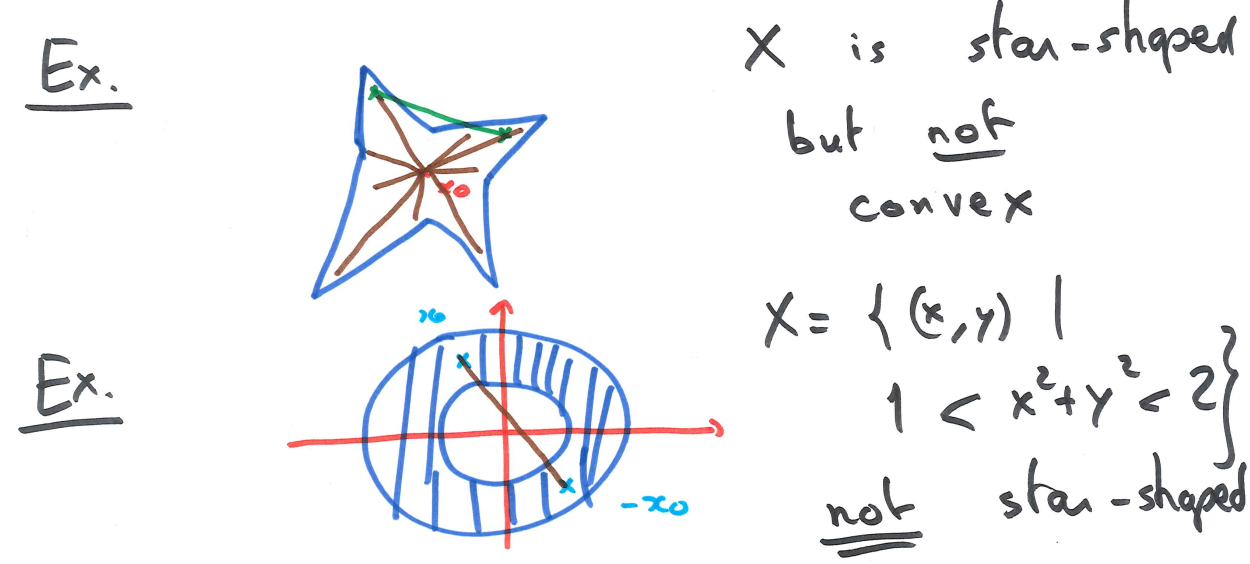
\includegraphics[width = 18em]{starshape}
    Konvex $\implies$ Sternförmig
\end{Definition}

\begin{Satz}{Sternförmig}{}
    Sei $X$ sternförmig und offen. Und $f$ ein $C^1$ Vektorfeld. Und 
    \[\frac{\partial f_i}{\partial x_j}=\frac{\partial f_j}{\partial x_i}\] auf X für alle $i \neq j$.
    Dann ist $f$ konservativ.

\end{Satz}

\begin{Definition}{Curl oder Rotation eines Vektorfeldes}{}
    Sie $X\subset \mathbb{R}^3$ und $f:X \rightarrow \mathbb{R}^3$ ein $C^1$ Vektorfeld.
    \[   
        \text{curl}(f) =
        \left(
        \begin{array}{c}
        \partial_{y}f_3 - \partial_zf_2\\
        \partial_zf_1 - \partial_x f_3\\
        \partial_xf2-\partial_yf_1\\
        \end{array}
        \right)
    \]
    Oder mittelhilfe det Determinante
    \[
        \text{curl}(f)=
        \begin{vmatrix}
        e_1 & e_2 & e_3\\
        \partial_x & \partial_y & \partial_z \\
        f_1 & f_2 & f_3\\
        \end{vmatrix}
    \]
\end{Definition}
\subsection{Das Riemann Integral}

\begin{Rechenregeln}{Riemann Integral}{}
    Das Riemann Integral über ein Quader $Q = [a_1,a_2] \times [a_2, b_2] \times \dots \times [a_n, b_n]$ wird mittel Partitionen Unter und Obersummen, wie im 1-Dimensionalen Fall definiert.
    Das Untere und Obere Riemann Integral ist:
    \[ 
        \int_{Q} f(x) d \mu=\underline{I}(f):=\sup \left\{U_{f}(P) \mid P \in \mathcal{P}(Q)\right\}
    \]
        
    \[
        \left(\text{resp ., } \int_{Q} f(x) d \mu=\bar{I}(f):=\inf \left\{O_{f}(P) \mid P \in \mathcal{P}(Q)\right\}\right)    
    \]
    $f$ heisst integrierbar wenn, $\bar{I}(f) = \underline{I}(f)$
\end{Rechenregeln}

\begin{Satz}{Eigenschaften des Riemann Integrals}{}
    \begin{enumerate}
        \def\labelenumi{\arabic{enumi}.}
        \item
          \textbf{Compatibility:} If \textbf{\(n=1\)} and \(X=[a,b]\) with
          \(a\leq b\), then \(\int_{[a,b]}f(x)dx=\int_a^bf(x)dx\).
        \item
          \textbf{Linearity:} If \(f\) and \(g\) are continuous on \(X\) and
          \(a,b \in \mathbb{R}\), then
          \(\int_X(af_1(x)+bf_2(x))dx = a\int_Xf_1(x)dx+b\int_Xf_2(x)dx\).
        \item
          \textbf{Positivity:} If \(f\leq g\), then
          \(\int_Xf(x)dx\leq\int_Xg(x)dx\) and especially, if \(f \geq 0\), then
          \(\int_Xf(x)dx \geq 0\). Moreover, if \(Y \subset X\) is compact and
          \(f\geq 0\), then \(\int_Yf(x)dx\leq\int_Xf(x)dx\).
        \item
          \textbf{Upper bound and triangle inequality:} In particular, since
          \(-|f|\leq f \leq |f|\), we have
          \(\left| \int_Xf(x)dx \right| \leq \int_X|f(x)|dx\), and since
          \(|f+g| \leq |f| + |g|\), we have
          \(\left| \int_X(f(x)+g(x))dx \right| \leq \int_X|f(x)|dx + \int_X|g(x)|dx\).
        \item
          \textbf{Volume:} If \(f=1\), then the integral of \(f\) is the
          \emph{volume} in \(\mathbb{R^n}\) of the set \(X\), and if \(f\geq 0\)
          in general, the integral of \(f\) is the volume of the set
          \(\{(x,y) \in X \times \mathbb{R} : 0 \leq y \leq f(x)\} \subset \mathbb{R}^{n+1}\).
          In particular, if \(X\) is a bounded \emph{rectangle}, say
          \(X = [a_1,b_1] \times ... \ \times [a_n, b_n] \subset \mathbb{R}^n\)
          and if \(f=1\), then \(\int_Xdx=(b_n-a_n) \cdot\cdot\cdot(b_1-a_1)\).
          We write $\text{Vol}(X)$
        \end{enumerate}
  
\end{Satz}
\begin{Satz}{Satz von Fubini}{}
    Reduzierung von mehrdimensionalen Integralen auf eine Dimension. Sei $f: [a,b] \times [c, d]$ stetig, dann gilt
    \[ \int_a^b dx \int_c^d f(x, y) dy = \int_c^d dy \int_a^b f(x, y) dx = \int\displaylimits_{[a,b] \times [c, d]} f(x, y) d\mu(x, y)   \]

    Es sei der Quader $Q = [a_1,a_2] \times [a_2, b_2] \times \dots \times [a_n, b_n]$ mit $f \in C^0(Q)$ gegeben. Dann gilt

    \[
        \int_Q f(x) d\mu(x) = \int_{a_1}^{b_1} dx_1 \int_{a_2}^{b_2} dx_2 \dots \int_{a_n}^{b_n} dx_n f(x_1, x_2,...,x_n)
    \]
    
    \textbf{Die Integrationsreihenfolge darf vertauscht werden.}
\end{Satz}

\begin{Definition}{Vernachlässigbare Mengen}{}
    \begin{enumerate}
        \def\labelenumi{\arabic{enumi}.}
        \item
          Let \(1\leq m \leq n\) be an integer. A parameterised \(m\)-set in
          \(\mathbb{R}^n\) is a continuous map
          \(f:[a_1,b_1]\times ...\ \times[a_m,b_m] \rightarrow \mathbb{R}^n\)
          which is \(C^1\) on \(]a_1, b_1[\ \times ... \times\ ]a_m,b_m[\).
        \item
          A subset \(B\subset \mathbb{R}^n\) is negligible if there exists an
          integer \(k \geq 0\) and parameterised \(m_i\)-sets
          \(f_i:X_1 \rightarrow \mathbb{R}^n\), with \(1\leq i \leq k\) and
          \(m_i < n\), such that \(X\subset f_1(X_1) \cup ...\ \cup f_k(X_k)\) .
        \item Satz: Wenn $X$ vernachlässigbar ist gilt:
            $\int_X f(x) dx = 0$
    \end{enumerate}
\end{Definition}
\begin{Definition}{Uneingentliche Integrale}{}
    Sei $X$ nicht kompakt. Und $X_k$ eine Reihe von kompakten Mengen sodass $X_k \subset X_{k+1}$ und
    $\cup_{k = 1}^{\infty} = X$. Dann konvergiert $\int_X f dx$ wenn
    \[
        \int_X f dx = \Lim{k \to \infty}{\int_X f dx}
    \]
    Im 2-Dimensionalen Fall, wenn die Anwendung von Fubini gleich ist.
\end{Definition}

\begin{Satz}{Substitutionsregeln in einer Dimension}{}
    Sei $f$ eine Riemann-integrierbare Funktion. Für die Berechnung des Integrals
    \[
        \int_a^b f(x) dx
    \]
    führt die Substitution $x \to g(u)$ zu $dx = g'(u)du$ und damit wird das Integral
    \[
        \int_a^b f(x) dx = \int_{g^{-1}(a)}^{g^{-1}(b)} f(g(u)) g'(u) du
    \]
    Das heisst wir haben das Integrationselement $dx$ durch $g'(u)du$ ersetzt und die Grenzen entsprechend angepasst.
\end{Satz}

\begin{Satz}{Substitutionsregel in $\R^2$}{}
    \[
        \int_{\Omega} f(x,y) ~ dx dy = \int_{\widetilde{\Omega}} f(g(u, v), \; h(u, v)) \, 
		    \left\lvert\det \, \underbrace{\begin{pmatrix}
			    \frac{\partial g}{\partial u} & \frac{\partial g}{\partial v}\\
			    \frac{\partial h}{\partial u} & \frac{\partial h}{\partial v}
		    \end{pmatrix}}_{d\Phi = \nabla\Phi} \right\rvert
	    ~ du dv
    \]
\end{Satz}

\begin{Satz}{Substitutionsregeln in $n$ Dimensionen}{}
    Sei $f$ eine Riemann-integrierbare Funktion auf dem Gebiet $\Omega \subset \R^n$ und die Koordinatentransformation (Substitution)
    \[
    (x_1,\hdots,x_n) = \Phi(u_1, \hdots,  u_n)
    \]
    oder in Komponenten
    \[
        \vek{x_1}{\vdots}{x_n}
        = \Phi(u)
        = \vek{g_1(u_1,\hdots,u_n)}{\vdots}{g_n(u_1,\hdots,u_n)}
    \]
    ist ein $C^1$-Diffeomorphismus. Dann gilt
    \[
        \int_\Omega f(x_1, \hdots, x_n)dx_1\hdots dx_1 = \int_{\widetilde{\Omega}} f(g_1(u), \hdots, g_n(u)) \cdot |\det d \Phi|\ du_1\hdots du_n
    \]
    wobei das Gebiet $\widetilde{\Omega} = \Phi^{-1}(\Omega)$ ist. $|\det d\Phi|$ ist die \textbf{Funktionaldeterminante} (Jakobi-Determinante).
\end{Satz}

\begin{Rechenregeln}{Koordinatentransformationen und Funktionaldet.}{}
	Wichtige Koordinatentransformationen und Funktionaldeterminanten\\
	
	Polarkoordinaten in $\R^2$
	\begin{alignat*}{4}
            x &= r \cos \varphi \quad &&0 \leq r < \infty \quad &&&dxdy = r \cdot drd\varphi\\
            y &= r \sin \varphi \quad &&0 \leq \varphi < 2\pi &&&
    \end{alignat*}
   	Elliptische Koordinaten $\R^2$
   	\begin{alignat*}{4}
            x &= r \cdot  a \cos \varphi\quad &&0 \leq r < \infty\quad &&&dxdy = a \cdot b \cdot  r \cdot drd\varphi\\
            y &= r \cdot b \sin \varphi\quad &&0 \leq \varphi < 2\pi &&&
   	\end{alignat*}
        Zylinderkoordinaten $\R^3$ \begin{alignat*}{4}
            x &= r \cdot  a \cos \varphi\quad &&0 \leq r < \infty &&&dxdydz = r \cdot drd\varphi dz\\
            y &= r \cdot b \sin \varphi\quad &&0 \leq \varphi < 2\pi\\
            z &= z\quad &&\-\infty \leq z < \infty\quad
    	\end{alignat*}
        Kugelkoordinaten $\R^3$ \begin{alignat*}{4}
            x &= r \cdot \sin \theta \cos \varphi \quad &&0 \leq r < \infty \quad &&&dxdydz = r^2 \sin \theta \cdot drd\theta d\varphi\\
            y &= r \cdot \sin \theta \sin \varphi \quad && 0 \leq \theta < \pi &&&\\
            z &= r \cos \theta \quad &&0 \leq \varphi < 2\pi &&&
        \end{alignat*}
\end{Rechenregeln}


\subsection{Geometrische Anwendungen von Integralen}

\begin{Rezept}{Area(D) - Vol(D) - Volumen eines Normalbereichs in $\R^n$}{}
Analog zum Integrieren über Normalbereich:
\[ \text{Vol}(D) = \int_D 1 ~ dX = \underbrace{\int \!\! \int \ldots \int}_{n} 1 ~ dx_1 \ldots dx_{n-1} dx_n,  ~~~~ D \subseteq \R^n\]
\end{Rezept}

\subsubsection{Normalbereiche in \texorpdfstring{$R^2$}{R2}}

\begin{Definition}{Normalbereiche in zwei Dimensionen}{}
Sei $\Omega$ eine beschränkte Teilmenge von $\R^2$. $\Omega$ heisst \textbf{y-Normalbereich}, falls sich $\Omega$ wie folgt darstellen lässt:

\[
    \Omega = \{(x, y) \in \R^2 \mid a \leq x \leq b, f(x) \leq y \leq g(x)\}
\]

wobei $f$, $g$ stetige Funktionen der Variable $x$ sind. Die Rolle von $x$ und $y$ darf vertauscht werden (es existiert also auch ein $x$-Normalbereich).

\includegraphics[width=.8\textwidth]{images/normalbereich}

(a): y-Normalbereich, (b): x-Normalbereich

\end{Definition}
\begin{Satz}{Integration auf Normalbereichen}{}

Sei \[\Omega = \{(x, y) \in \R^2 \mid a \leq x \leq b, f(x) \leq y \leq g(x)\}\] ein \textbf{y-Normalbereich} mit stetigen Funktionen $f$, $g$ und sei die zu integrierende Funktion $F \in C^0(\Omega)$, dann gilt:

\[
    \int_{\Omega} F d\mu = \int_a^b dx \int_{f(x)}^{g(x)} dy F(x, y)
\]

Das innere Integral wird zuerst ausgewertet.
\end{Satz}

\begin{Rezept}{Integrieren über Normalbereichen}{}
Am folgenden Beispiel:
\[ \int_D f(x, y) ~ dx dy ~~ \text{ wobei } ~~ D = \R^2 \cap \{(x, y) ~ | ~ y \geq 0 ~ \wedge ~ x-y+1\geq 0 ~ \wedge ~ x+2y-4 \leq 0\}\]
\begin{enumerate}
\item {
Es hilft, sich den Normalbereich visuell vorzustellen, um die Grenzen
zu finden. Bedingungen nutzen:
\[ y \geq 0 ~ \wedge (y-1 \leq x \leq 4-2y) \]
Damit $x$ nicht leer ist, muss $y-1 \leq 4-2y$ sein, resp. $y \leq \frac{5}{3}$ 
}
\item {
Für das äussere Integral sind die Integrationsgrenzen nun fest vorgegeben. Die inneren Grenzen
werden abhängig von der äusseren Variable gewählt:

\[ \int_D f(x,y) ~ dx dy = \int_0^{\frac{5}{3}} \int_{y-1}^{4-2y} f(x,y) ~ dx dy \]

}
\end{enumerate}
\end{Rezept}

\subsubsection{Satz von Green}

Dieser Satz erlaubt uns, eindimensionale Wegintegrale in zweidimensionale Gebietsintegrale umzuwandeln. D.h. wir rechnen dann jeweils die Variante aus, die einfacher geht.
Idee: Beziehung Linienintegral und Flächenintegral.


\begin{Satz}{Satz von Green in der Ebene}{}
	Sei $\vec{v} = (v_1, v_2)$ ein stetig differenzierbares Vektorfeld auf einem Gebiet $\Omega \subset \R^2$ und $C \subset \Omega$ ein beschränkter Bereich mit $C^1_{pw}$ Rand $\partial C$, der sich nicht selbst schneidet. Dann gilt
	\[
		\int_{\gamma=\partial C} \vec{v} \cdot d\vec{s} = 
		\int_C \left(\frac{\partial v_2}{\partial x} - \frac{\partial v_1}{\partial y}\right) dxdy
	\]
	Wenn die Region durch eine Vereinigung von Kurven eingeschlossen ist:\\
	\[
		\displaystyle\int_X\left(\frac{\partial f_2}{\partial x}-\frac{\partial f_1}{\partial y}\right)dxdy = \sum_{i=1}^k\int_{\gamma_i}f\cdot d\vec s	
	\]
	\textbf{Bemerkung I}: Der Rand $\partial C$ muss im positiven mathematischen Sinn durchlaufen werden. D.h. das Gebiet $C$ muss jeweils links vom Rand sein, für ein Beobachter, der auf dem Rand läuft.\\
	
	\textbf{Bemerkung II}: Der Satz von Green ist die zweidimensionale Version des Satzes von Stokes
	
	\textbf{Bemerkung III}: $\gamma=\partial C$ muss den gesamten Rand abdecken. Evtl. Gebietsadditivität nutzen und gewisse Bereiche (Ränder) einzeln parametrisieren.
\end{Satz}

\begin{Definition}{Divergence}{}
	Sie $f: \mathbb{R}^n \rightarrow \mathbb{R}^n$ ein Vektorfeld, die divergence ist
	\[
		\text{div} f = \partial x_1 + ... + \partial x_n
	\]
\end{Definition}

\begin{Satz}{Green andere Formen}{}
	\[
	\int_X \int	div f dx dy = \int_{\partial X} f_0 d\vec n
	\]
	\[
		\int_X \int	curl f dx dy = \int_{\partial X} \vec f \vec ds
	\]
\end{Satz}

\begin{Rezept}[label=GreenFlaechen]{Flächen berechnen mit Satz von Green}{}
	Gegeben: Gebiet $C \subset \R^2$ beschränkt mit $C^1_{pw}$ Rand $\partial C$.
	
	Gesucht: Fläche $F(C)$\\
	
	\textbf{Lösungsschritt I}:
	
	Parametrisiere den Rand von C mit einer Kurve
	\[
  		\gamma:[a, b] \to \R^2,\quad t \mapsto \gamma(t)
	\]
	Beachte, dass die Parametrisierung in positiver mathematischer Richtung verläuft. D.h. das Gebiet muss jeweils links der Kurve sein.
	
	\textbf{Lösungsschritt II}:
	
	Berechne $\gamma'$

	\textbf{Lösungsschritt III}:
	
	Wähle ein geeignetes Vektorfeld:
	$\frac{\partial v_2}{\partial x} -\frac{\partial v_1}{\partial y} = 1$ 
	Zum Beispiel $\vec v = (0, x)$ oder $\vec v = (-y/2, x/2)$ oder $\vec v = (-y, 0)$.
	Wende dafür den Satz von Green an,
	\[
  		F(C) =
  		\int_{\gamma=\partial C} \vec{v} \cdot d\vec{s}
	\]
\end{Rezept}

\begin{Satz}{Masse und Schwerpunkt und Oberfläche}{}
	Sei $\Omega$ ein zweidimensionales Gebiet mit Massendichte $\rho(x, y)$, welche die Massenverteilung auf $\Omega$ beschreibt. Die \textbf{Masse} von $\Omega$ ist dann	
	\[
		M(\Omega) = \int_\Omega \rho(x, y) dx dy
	\]
	Der \textbf{Schwerpunkt} $S=(x_s, y_s)$ von $\Omega$ ist gegeben durch
	\begin{align*}
		x_s &= \frac{1}{M} \int_\Omega x \rho (x, y) dx dy\\
		y_s &= \frac{1}{M} \int_\Omega y \rho (x, y) dx dy
	\end{align*} 
	Analog berechnen sich Masse, Schwerpunkt von dreidimensionalen Gebieten.\\
	Oberfläche: Consider the continuous function
	\(f:[a,b] \times [c,d] \rightarrow \mathbb{R}\) which is \(C^1\) on
	\(]a,b[\times]c,d[\). Let
	\(\Gamma = \{(x,y,z) \in \mathbb{R}^3 : (x,y) \in [a,b]\times [c,d], z=f(x,y)\} \subset\mathbb{R^3}\)
	be the graph of \(f\). This is a surface and should have an area, which
	is given by
	\(\int_a^b\int_c^d\sqrt{1+(\partial_xf(x,y))^2+(\partial_yf(x,y))^2}dxdy\)
	Analogue formula for the length of the graph of a function $f:[a,b] \rightarrow \mathbb{R}$: $\int_a^b\sqrt{1+f'(x)^2}dx.$
\end{Satz}
\begin{Satz}{Satz von Stokes}{}
	Sei $\vec{v} = (v_1, v_2, v_3)$ ein stetig differenzierbares Vektorfeld auf $\Omega \subset \R^3$ und $C \subset \Omega$ eine offene Fläche durch die geschlossene $C^1_{pw}$ Kurve $\gamma = \partial C$ berandet:
	\[
		\int_{\gamma=\partial C} \vec{v} \cdot d\vec{s} = 
		\int_C (\vec \nabla \times \vec v) \cdot \vec n\ do
	\]
	wobei $\vec n$ der nach aussen gerichtete Normalenvektor entlang $C$ und $do$ das zweidimensionale Integrationselement über die Fläche bezeichnen. Der Weg $\gamma$ muss positiv orientiert sein.	
	
\end{Satz}

\subsubsection{Satz von Gauss}

\begin{Satz}{Satz von Gauss}{}
	Sei V ein beschränkter räumlicher Bereich mit Rand $\partial V \in C^1_{pw}$ gegeben. Sei das Vektorfeld $\vec v$ auf ganz $V$ definiert und stetig differenzierbar. Dann gilt
	\[
		\int_{\partial V} \vec v \cdot \vec n\ do = \int_V \vec \nabla \cdot \vec v\ d \mu
	\]
	wobei $\vec n$ der nach aussen gerichtete Normalenvektor entlang $\partial V$, $do$ das zweidimensionale Integrationselement über die Fläche und $d\mu$ das dreidimensionale Integrationselement über das Volumen bezeichnen.
\end{Satz}
 
\input{content/4_tricks.tex}

%% (c) 2019 Oliver Senn

\section{Integrale}
\subsection{Spezielle unbestimmte Integrale}
$\mathlarger{\int (ax+b)^s\;dx= \frac{1}{a(s+1)}(ax+b)^{s+1} + C,\;s\neq -1}$\\
$\mathlarger{\int \frac{1}{ax+b}dx=\frac{1}{a}\;log|ax+b|+C}$\\
$\mathlarger{\int (ax^p+b)^sx^{p-1}\;dx = \frac{(ax^p+b)^{s+1}}{ap(s+1)}+C,\;s\neq -1, a \neq 0}$\\
$\mathlarger{\int (ax^p+b)^{-1}x^{p-1}\;dx=\frac{1}{ap}log|ax^p+b|+C,\;a\neq 0,p\neq 0}$\\
$\mathlarger{\int \frac{ax+b}{cx+d}dx=\frac{ax}{c}- \frac{ad-bc}{c^2} log|cx+d|+C}$\\
$\mathlarger{\int \frac{1}{x^2+a^2}dx=\frac{1}{a}arctan(\frac{x}{a})+C}$\\
$\mathlarger{\int \frac{1}{x^2-a^2}dx=\frac{1}{2a}log\Bigl|\frac{x-a}{x+a}\Bigl|}$\\
$\mathlarger{\int \sqrt{a^2+x^2}\;dx=\frac{x}{2}\sqrt{a^2+x^2}+\frac{a^2}{2} log(x+\sqrt{a^2+x^2})+C}$\\
$\mathlarger{\int \sqrt{a^2-x^2}\;dx= \frac{x}{2}\sqrt{a^2-x^2}+\frac{a^2}{2}arcsin\Bigl(\frac{x}{|a|}\Bigl)+C}$\\
$\mathlarger{\int \sqrt{x^2-a^2}\;dx= \frac{x}{2}\sqrt{x^2-a^2}-\frac{a^2}{2}log|x+\sqrt{x^2-a^2}|+C}$\\
$\mathlarger{\int \frac{1}{\sqrt{x^2-a^2}}\;dx=log(x+\sqrt{a^2+x^2})+C}$\\
$\mathlarger{\int \frac{1}{\sqrt{x^2-a^2}}\;dx=log|x+\sqrt{x^2-a^2}|+C}$\\
$\mathlarger{\int \frac{1}{\sqrt{a^2-x^2}}\;dx=arcsin\Bigl(\frac{x}{|a|}\Bigl)+C}$\\
$\mathlarger{\int e^{kx}\;dx=\frac{1}{k}e^{kx}+C}$\\
$\mathlarger{\int a^{kx}\;dx=\frac{1}{k*log(a)}a^{kx}+C}$\\
$\mathlarger{\int e^{ax}p(x)\;dx=e^{ax}(a^{-1}p(x)-a^{-2}p'(x)+a^{-3}p''(x)-\dots}$\\
$\mathlarger{+(-1)^na^{-n-1}p^{(n)}(x))+C}$, $a\neq 0$, p: Polynom n-ten Grades\\
$\mathlarger{\int e^{kx}sin(ax+b)\;dx=\frac{e^{kx}}{a^2+k^2}\Bigl(k\;sin(ax+b)- a\;cos(ax+b)\Bigl)+C}$\\
$\mathlarger{\int e^{kx}cos(ax+b)\;dx=\frac{e^{kx}}{a^2 + k^2}\Bigl(k\;cos(ax+b)...}$\\
$\mathlarger{...+a\;sin(ax+b)\Bigl)+C}$\\
$\mathlarger{\int log|x|\;dx= x(log|x|-1)+C}$\\
$\mathlarger{\int x^k log(x)\;dx=\frac{x^{k+1}}{k+1}\Bigl(log(x)-\frac{1}{k+1}\Bigl)+C}$, $k\neq -1$\\
$\mathlarger{\int x^{-1}log(x)\;dx= \frac{1}{2}(log(x))^2 + C}$\\
$\mathlarger{\int sin(ax+b)\;dx=-\frac{1}{a}cos(ax+b)+C}$\\
$\mathlarger{\int cos(ax+b)\;dx=\frac{1}{a}sin(ax+b)+C}$\\
$\mathlarger{\int sin^2(x)\;dx= \frac{1}{2}(x-sin(x)cos(x))+C}$\\
$\mathlarger{\int cos^2(x)\;dx= \frac{1}{2}(x+sin(x)cos(x))+C}$\\
$\mathlarger{\int tan^2(x)\;dx= tan(x)-x+C}$\\
$\mathlarger{\int \frac{1}{sin(x)}\;dx=log\Bigl|tan\frac{x}{2}\Bigl|+C}$\\
$\mathlarger{\int \frac{1}{cos(x)}\;dx=log\Bigl|tan\Bigl(\frac{x}{2}+\frac{\pi}{4}\Bigl)\Bigl|+C}$\\
$\mathlarger{\int \frac{1}{tan(x)}\;dx=log|sin(x)|+C}$\\


\subsection{Spezielle bestimmte Integrale}
$\mathlarger{\int_0^{2\pi} sin(mx)cos(nx)\;dx=0}$, $m,n\in \mathbb{Z}$\\
$\mathlarger{\int_0^\infty \frac{sin(ax)}{x}\;dx=\frac{\pi}{2},\;a>0}$\\
$\mathlarger{\int_0^\infty sin(x^2)\;dx=\int_0^\infty cos(x^2)\;dx=\frac{1}{2}\sqrt{\frac{\pi}{2}}}$\\
$\mathlarger{\int_0^\infty e^{-ax}x^n\;dx= \frac{n!}{a^{n+1}},\;a>0}$\\
$\mathlarger{\int_0^\infty e^{-ax^2}\;dx=\frac{1}{2}\sqrt{\frac{\pi}{a}},\;a>0}$\\


\end{document}
